\documentclass[sigconf,review,anonymous]{acmart}

%%
%% \BibTeX command to typeset BibTeX logo in the docs
\AtBeginDocument{%
  \providecommand\BibTeX{{%
    Bib\TeX}}}

\setcopyright{none}
\settopmatter{printacmref=false}
\renewcommand\footnotetextcopyrightpermission[1]{} % removes footnote with conference information in first column

%\setcopyright{acmcopyright}
% \setcopyright{none}
\copyrightyear{2018}
\acmYear{2018}
\acmDOI{XXXXXXX.XXXXXXX}

%% These commands are for a PROCEEDINGS abstract or paper.
\acmConference[ICSE 2024]{46th International Conference on Software Engineering}{April 2024}{Lisbon, Portugal}
%%
%%  Uncomment \acmBooktitle if the title of the proceedings is different
%%  from ``Proceedings of ...''!
%%
%%\acmBooktitle{Woodstock '18: ACM Symposium on Neural Gaze Detection,
%%  June 03--05, 2018, Woodstock, NY}
\acmPrice{15.00}
\acmISBN{978-1-4503-XXXX-X/18/06}

% \settopmatter{printacmref=false}

%% Some recommended packages.
\usepackage{booktabs}   %% For formal tables:
                        %% http://ctan.org/pkg/booktabs
\usepackage{subcaption} %% For complex figures with subfigures/subcaptions
                        %% http://ctan.org/pkg/subcaption

\usepackage[utf8]{inputenc}
\usepackage[T1]{fontenc}
\usepackage[scaled=0.8]{beramono}
\usepackage{amsmath}
\usepackage{color}
\usepackage{xcolor,colortbl}
\usepackage{url}
\usepackage{listings}
\usepackage{paralist}
\usepackage{caption}
\usepackage{wrapfig}
\usepackage{enumitem}
\usepackage{multicol}
\usepackage{flushend}
\usepackage{bcprules}
\usepackage{textcomp}
\usepackage{pdfpages}
\usepackage{cleveref}
\usepackage{xspace}
\usepackage{stackengine}
\usepackage{stmaryrd}
\usepackage{multirow}
\usepackage{xurl}

\definecolor{light-gray}{gray}{0.85}
% ----- listings

\definecolor{light-gray}{gray}{0.85}
%\definecolor{ckeyword}{HTML}{7F0055}
\definecolor{ckeyword}{HTML}{000000}
\definecolor{ccomment}{HTML}{3F7F5F}
\definecolor{cstring}{HTML}{2A0099}

\colorlet{shadecolor}{light-gray!40}

\lstdefinelanguage{Solidity}%
{morekeywords = {
  abstract, contracts, is,
  ether, szabo, finney, wei,
  seconds, minutes, hours, days, weeks, years,
  function, constructor, memory, calldata,
  for, if, new
  mapping,
  internal, external, pure, view, payable, return, returns,
  public, private, virtual, override,
  true, false, bool,
  bytes, bytes32,
  uint, uint8, uint16, uint32, uint64, uint128, uint256,
  int, int8, int16, int32, int64, int128, int256,
  address, string,
  require, assert, revert, try, catch,
  requires, ensures, where
  },%
  sensitive,%
  %identifierstyle = \color{blue},
  moredelim = *[l][\itshape]{\#},
  morecomment = [l]//,%
  morecomment = [s]{/*}{*/},%
  morestring = [b]",%
  %morestring=[b]',%
  showstringspaces = false%
}[keywords,comments,strings]%

\lstset{
  language=Solidity,%
  backgroundcolor=\color{shadecolor},%
  mathescape=true,%
%  columns=[c]fixed,%
  aboveskip=2pt,%\smallskipamount,
  belowskip=1pt,%\negsmallskipamount,
  lineskip=-1pt,
  basewidth={0.6em, 0.5em},%
%  backgroundcolor=\color{listingbg},
  basicstyle=\ttfamily\small,
  keywordstyle=\keywordstyle,
  commentstyle=\commentstyle,
  stringstyle=\stringstyle,
%  xleftmargin=0.5cm
  literate={-->}{{$\to$}}2
           {->}{{$\mapsto$}}3
           {<-}{{$\leftarrow$}}2
           {=>}{{$\Rightarrow ~$}}2
           {=/>}{{$\not\Rightarrow ~$}}3
           {~>}{{$\leadsto$}}2
           {~/>}{{$\not\leadsto$}}2
           {|-}{{$\ts$}}2
           {σ}{{$\sigma$}}1
           {ρ}{{$\rho$}}1
           {→}{{$\to$}}1
           {←}{{$\leftarrow$}}1
           {λ}{{$\lambda$}}1
           {α}{{$\alpha$}}1
           {⊔}{{$\sqcup$}}1
           {⊓}{{$\sqcap$}}1
           {⊑}{{$\sqsubseteq$}}1
           {⊤}{{$\top$}}1
           {⊥}{{$\bot$}}1
           {×}{{$\times$}}1
           {τ}{{$\tau$}}1
           {ψ}{{$\psi$}}1
           {Σ}{{$\Sigma$}}1
           {⟨}{{$\langle$}}1
           {⟩}{{$\rangle$}}1
           {π}{{$\pi$}}1
           {∪}{{$\cup$}}2
           {/\\}{{$\land$}}2
           %{[[}{{$[\![$}}1
           %{]]}{{$]\!]$}}1
           %{…}{{$\!...$}}1
}

\definecolor{listingbg}{RGB}{240, 240, 240}

\newcommand{\commentstyle}[1]{\color{ccomment}\itshape{#1}}
\newcommand{\keywordstyle}[1]{\color{ckeyword}\bfseries{#1}}
\newcommand{\stringstyle}[1]{\color{cstring}\text{#1}}

\lstnewenvironment{listing}{\lstset{language=Solidity}}{}
\lstnewenvironment{listingtiny}{\lstset{language=Solidity,basicstyle=\scriptsize\ttfamily}}{}

\newcommand{\code}[1]{\lstinline[language=Solidity,columns=fixed,basicstyle=\ttfamily]|#1|}

\renewcommand{\paragraph}[1]{\vspace{0.15em}\noindent\textit{\textbf{#1.}}}

% ----- formal

\newcommand{\judgement}[2]{{\bf #1} \hfill #2}
\newcommand{\den}[1]{\llbracket~#1~\rrbracket}

% ----- comments and todo

\newcommand{\note}[1]{{\color{red}[#1]}}
\newcommand{\todo}[1]{\note{TODO: #1}}
\newcommand{\wac}[1]{{\color{orange}[WAC: #1]}} % Wuqi's comment
\newcommand{\zz}[1]{{\color{blue}[ZZ: #1]}} % ZZ's comment
\newcommand{\yy}[1]{{\color{Plum}[YY: #1]}} % YY's comment
\newcommand{\rev}[1]{\note{Revision: #1}}
\newcommand{\silent}[1]{}
\newcommand{\hl}[1]{\setlength{\fboxsep}{0pt}\colorbox{light-gray}{#1}}

\newcommand{\lang}{\textsc{ConSol}\xspace}
\newcommand{\corelang}{$\lambda_\lang$\xspace}

\newcommand{\lb}{\{~}
\newcommand{\rb}{~\}}
\newcommand{\la}{\langle}
\newcommand{\ra}{\rangle}

\newcommand{\Typ}[1]{\ensuremath{\mathsf{#1}}}
\newcommand{\Keywd}[1]{\ensuremath{\texttt{#1}}}
\newcommand{\Ast}[1]{\ensuremath{\mathsf{#1}}}
\newcommand{\Def}[1]{\ensuremath{\mathsf{#1}}}

% ----- syntax
\newcommand{\optional}[1]{{\color{gray}\left[{\color{black}#1}\right]}}
\newcommand{\state}{\sigma} % global state of all contracts
\newcommand{\store}[1]{\delta_{#1}} % state of a individual contract

\newcommand{\addr}{\mathcal{A}}
\newcommand{\bddr}{\mathcal{B}}
\newcommand{\cddr}{\mathcal{C}}
\newcommand{\dddr}{\mathcal{D}}
\newcommand{\xddr}{\mathcal{X}}
\newcommand{\yddr}{\mathcal{Y}}
\newcommand{\sender}{\mathtt{sender}}

% ------ semantics
\newcommand{\denot}[1]{\llbracket#1\rrbracke}


\begin{document}

%\title{Contracts for Contracts \\
%  {\Large Securing Smart Contracts with Higher-Order Temporal Behavioral Contracts}
%}

\title{Consolidating Smart Contracts with Behavioral Contracts}

\author{Ben Trovato}
\authornote{Both authors contributed equally to this research.}
\email{trovato@corporation.com}
\orcid{1234-5678-9012}
\author{G.K.M. Tobin}
\authornotemark[1]
\email{webmaster@marysville-ohio.com}
\affiliation{%
  \institution{Institute for Clarity in Documentation}
  \streetaddress{P.O. Box 1212}
  \city{Dublin}
  \state{Ohio}
  \country{USA}
  \postcode{43017-6221}
}

\iffalse
\lstMakeShortInline[keywordstyle=,%
  flexiblecolumns=false,%
  %basewidth={0.56em, 0.52em},%
  mathescape=false,%
  basicstyle=\ttfamily\small]@
\fi

\begin{abstract}
  Ensuring the reliability of smart contracts is of vital importance.
  However, existing static and dynamic verification tools are not expressive 
  or convenient enough for many rich properties.
  Moreover, as part of the programming tool, they do not offer programmers a notion 
  to articulate the interface between components.
  We argue that the ``design-by-contract'' approach should complement the development
  of smart contract programs. Unfortunately, there is only minimal linguistic support
  in existing smart contract languages.

  In this paper, we introduce a Solidity language extension \lang that supports
  behavioral contracts. \lang offers programmers a modular specification
  and monitor system for both first-order and higher-order behaviors. % (e.g. functions taking addresses as arguments).
  %We describe \lang with examples, static semantics, and translation semantics.
  We evaluate \lang using \numCaseStudied real-world cases, showing 
  the effectiveness of \lang 
  % that our approach is effective 
  in expressing critical conditions and preventing attacks.
  % Using 33 cases, w
  We also evaluate \lang's efficiency and compare the gas consumption with manually inserted assertions,
  % their gas consumption of \lang  compared to manually inserted assertions,
  showing that our approach only introduces minimal gas overhead.
  By separating specifications and implementations, \lang helps programmers 
  write not only more robust but also more readable code.
  
  %\lang offers an appealing approach to building robust smart contract
  %programs without sacrificing readability and maintainability.
  
\end{abstract}

%%
%% The code below is generated by the tool at http://dl.acm.org/ccs.cfm.
%% Please copy and paste the code instead of the example below.
%%
\iffalse
\begin{CCSXML}
<ccs2012>
 <concept>
  <concept_id>10010520.10010553.10010562</concept_id>
  <concept_desc>Computer systems organization~Embedded systems</concept_desc>
  <concept_significance>500</concept_significance>
 </concept>
 <concept>
  <concept_id>10010520.10010575.10010755</concept_id>
  <concept_desc>Computer systems organization~Redundancy</concept_desc>
  <concept_significance>300</concept_significance>
 </concept>
 <concept>
  <concept_id>10010520.10010553.10010554</concept_id>
  <concept_desc>Computer systems organization~Robotics</concept_desc>
  <concept_significance>100</concept_significance>
 </concept>
 <concept>
  <concept_id>10003033.10003083.10003095</concept_id>
  <concept_desc>Networks~Network reliability</concept_desc>
  <concept_significance>100</concept_significance>
 </concept>
</ccs2012>
\end{CCSXML}

\ccsdesc[500]{Computer systems organization~Embedded systems}
\ccsdesc[300]{Computer systems organization~Redundancy}
\ccsdesc{Computer systems organization~Robotics}
\ccsdesc[100]{Networks~Network reliability}
\fi

%\keywords{smart contracts, behavioral contracts, specification, runtime verification}

\maketitle

\section{Introduction} \label{sec:intro}

%https://se.inf.ethz.ch/~meyer/publications/old/dbc_chapter.pdf
%https://docs.soliditylang.org/en/v0.8.17/control-structures.html?highlight=require#panic-via-assert-and-error-via-require

%\todo{why? solidity is rather flexible, unsatisfying/weaker type system,
%not all invariants can be checked statically, e.g. the status of the chain}
%One \note{common} use case of higher-order functions in smart contracts is
%to express callback \todo{explain how it is used}.

%\todo{it is hard to enforce properties when callbacks exist}
%Static verification cannot completely address the issue here since
%transaction developers are oblivious to the user-provided callback.

%Building trustworthy and secure smart contract programs requires solid
%understanding and reliable enforcement of program invariants.

Smart contracts are programs to automate the execution of transactional agreements, ensuring that all involved parties align in their expectations of the outcome. 
% to automate the execution of transactional  agreements so that all parties involved in the agreement can be certain  about the outcome.
% Deployed on blockchains, immutable and distributed ledgers~\cite{nakamoto2008bitcoin}, these programs 
% uphold the principles of 
% immutable, distributed ledgers~\cite{nakamoto2008bitcoin}, and 
% Smart contract 
Smart contract programs are ``smart'' as they
% since they are programs to 
% therefore  
\emph{ensure the economic outcome of transactions} by running on decentralized blockchains, 
implementing a consensus protocol of immutable, distributed ledgers \cite{nakamoto2008bitcoin}.
% By using blockchains,
Since transactions cannot be amended or revoked once finalized on the blockchain,
the reliability of smart contract programs is of vital importance, especially
for those involving financial or monetary operations.
%Due to the immutability of transactions,
% , these smart contracts, 
%once deployed\todo{another word}, they cannot be amended or undone. 
%Given that smart contracts are extensively utilized in financial operations, their reliability and security are of vital importance. %\xx{revised}
%\xx{no reverse back + transactions, therefore the reliability and security of smart contracts are of vital importance..}


It is however ironic that despite the potential of smart contracts,
\emph{languages} writing smart contracts often lack adequate mechanisms to \emph{ensure the
computational outcomes}. This unfortunate reality results in an unsatisfactory
quality of smart contract programs. Without proper means to ensure the quality
of these programs, the aspiration to ensure the economic outcome of
transactions remains nothing more than a mere wish.

Undoubtedly, the past few years have witnessed several catastrophic failures
of blockchain systems resulting from attacks on vulnerable contract programs \cite{DBLP:conf/icse/ZhangZXL23}.
One prominent instance is the well-known DAO hack~\cite{DAOhack} where an unauthorized
attacker exploited recursive function calls and callback mechanisms, leading
to a staggering loss of \textdollar50 million. The fundamental issue at the core of this
attack on deployed contracts was the failure to prevent reentrancy under certain 
critical conditions.

%\zz{ On the other hand, assertion primitives are crucial for ensuring the
%accuracy and integrity of a smart contract's business model. }
%\zz{ I'm not sure if this statement applies to the PL community, but from my
%understanding, assertions are typically used during testing rather than
%runtime.  However, in smart contracts, these assertions function as guard
%conditions and can cause reverts if violated, making them extremely important. }

%Solidity also provides the @modifier@ mechanism that intercepts
%before and after a function call, thus can be used to check
%pre- and post-conditions.
%\todo{can we compose modifier?}
%\todo{can we attach modifier to callbacks?}
%\todo{can we use modifier to check function's argument?}

\iffalse
\begin{figure}[t]
\begin{lstlisting}[numbers=left,stepnumber=1,xleftmargin=1em,numberstyle=\ttfamily\color{gray},numbersep=3pt]
interface IERC20 {
  function transferFrom(address, address, unit);
}
contract Vault {
  address owner;
  constructor() { owner = msg.sender; }
  function deposit(address token, uint amount) public {
    require(msg.sender == owner);
    IERC20(token).transferFrom(msg.sender, 
      address(this), amount);
  }
}
\end{lstlisting}
\caption{A simplified example using addresses. \note{GW: this is an important example, mentioned in sec 1/2/3, should think about ways to improve}
\todo{GW: DAO?} \todo{GW: explain this with more details}
}
\label{fig:intro_example}
\end{figure}
\fi

To prevent such attacks, programmers need to specify those critical
conditions. The execution is allowed only when those conditions are met.
However, we observe that existing popular smart contract languages (e.g.,
Solidity) do not provide \emph{expressive, effective, and convenient} means to
\emph{specify} and \emph{enforce} contract behaviors.
Static verification techniques have been intensively investigated (e.g. \cite{DBLP:journals/pacmpl/AlbertGRRRS20,
DBLP:journals/pacmpl/SmaragdakisGLTT21, DBLP:journals/pacmpl/SmaragdakisGLTT21, DBLP:journals/pacmpl/TanMLDF22}),
but they are often expensive or imprecise \cite{rice1953classes} to use in practice.
Run-time validations such as simple assertions of primitive data are available, 
but they are inconvenient to use and ineffective at 
% they are neither convenient to use, nor can effectively 
examining values carrying computational content. % \xx{cite and example}. 
For example, callable addresses and functions, as common patterns used in developing
smart contract programs, introduce higher-order behaviors \emph{when used as arguments} %\xx{example, explain figure with details}
(\Cref{fig:sturby_buggy} for an example) and often exhibit elusive vulnerabilities. % \xx{example}. 
%Moreover, many of the critical conditions in smart contracts are \emph{temporal}
%-- the order of events matters.
%For instance, to defense the DAO attack caused by reentrancy via
%external functions, it requires to check that the function of interest cannot
%be invoked \emph{before} the current call of the same function is finished.

%\xx{without effective tools or proper ways, developers tend to write error-prong assertions which are inconvenient. This urges the need to have sufficient linguistic means to provide expressive, effective and convenient way to guard the contracts and xxx. However, they do not exist. }

The lack of \textit{sufficient  linguistic means} to modularly specify and enforce 
subtle and critical behaviors discourages programmers from writing clean and maintainable
code with higher-level abstractions.
Instead, programmers are obliged to meticulously write verbose low-level code (e.g. assertions)
to implement defensive checks. These checks are interspersed with the main business logic,
 leading to poor readability and maintainability 
(\Cref{fig:sturby_buggy}).
%The pervasive temporal conditions in distributed blockchain systems further
%complicates the situation: these temporal behavioral checks are usually
%encoded as value-level checks in ad-hoc manners.
%Taking the DAO attack as example again, a common way to implement ``reentrancy
%guards'' is to manually define an additional boolean flag, indicating
%whether the function is finished. This is both verbose and error-prone,
%quickly becoming unmanageable for complex behaviors.
Often worse, defensive checks are neglected, resulting in
vulnerable code causing real monetary loss.
%\todo{DX: need a concrete motivating example?}
% GW: yes

%Apart from the investigating effort to certify and verify smart contract
%programs, language designers are responsible to empower programmers with better
%linguistic solutions to secure smart contracts in the first place.
% \subsubsection*{\textbf{Raise the Level of Expressiveness}}
\bfpara{Raise the Level of Expressiveness.}
To address these issues, we argue that \emph{behavioral software
contracts}~\cite{DBLP:conf/tools/Meyer98a} should play a fundamental role in
the development of reliable \emph{smart contract} programs.
As a metaphor, ``behavioral contracts'' specify assumptions and guarantees 
between software components, just as ``smart contracts'' specify assumptions and guarantees 
between business parties.
The two notions of ``contract'' should complement each other.
%\xx{why is this similarity important?}

Behavioral contracts are an expressive and convenient tool for programmers since assumptions (pre-conditions) and guarantees (post-conditions)
are specified as executable specifications, written in the same programming language syntax.
%\xx{therefore offers convenient and expressive ways to ..(why appealling)}.
At run-time, violations of these conditions are monitored and reported.
Studies \cite{DBLP:conf/rodin/Chalin06, DBLP:books/ph/Meyer97}
have shown that behavioral contracts can effectively support design, development,
testing, and debugging of software systems.
Pioneered by the Eiffel language \cite{DBLP:books/ph/Meyer91},
programmers have embraced the design-by-contract methodology \cite{DBLP:conf/tools/Meyer98a,
DBLP:books/ph/Meyer97} to build high-assurance software in various languages 
with extensions of behavioral contracts,
e.g., Java \cite{DBLP:journals/sttt/BurdyCCEKLLP05},
C++ \cite{boost_contract},
Python \cite{icontract},
Haskell \cite{DBLP:conf/popl/XuJC09},
Racket \cite{DBLP:conf/icfp/FindlerF02},
Elixir \cite{DBLP:conf/erlang/0001BBHMEF22}, etc. 

Unfortunately, such expressive tools for smart contract programmers are not yet available. %\xx{to fill the gap}
In this paper, we offer the first behavioral contract system \lang \footnote{\emph{Con}tract \emph{Sol}idity, or, \emph{Con}solidating \emph{Sol}idity.}, providing a practical
specification and monitoring system for Solidity, the most widely-used smart contract language, of both  \textit{first-order} and \textit{higher-order} behaviors.
% for the most widely-used smart contract language, Solidity.
\begin{itemize}[leftmargin=0.3cm, topsep=1.5pt]
% [leftmargin=2em]
  \item \lang is \emph{non-intrusive}, i.e., it does not alter either static or dynamic behaviors of Solidity programs.
  \item \lang is \emph{effective}, i.e., it monitors violations of specified conditions for both top-level functions and address calls, regardless of how the address value flows in the program.
  \item \lang is \emph{expressive}, i.e., programmers can liberally write and enforce any computable properties.
  \item \lang is \emph{gradual}, i.e., programmers only write specifications when necessary.
  \item \lang is \emph{efficient}, i.e., incurring minimal monitoring overhead (gas consumption) at run-time.
\end{itemize}
\lang enables the development of smart contract programs that are more reliable, readable, and maintainable. 
% writing not only more reliable, but also more readable and
% maintainable smart contract programs.
We then discuss the two main features of \lang.
%\xx{the benefit of \lang is threefold. 1. effective for both first-order and higher-order and persistent monitoring on the addresses 2. expressive  (ANY properties) 3. convenient no need to learn new languages, and offers great readability and maintainability. }

%\lang enriches the Solidity language with \emph{higher-order} and
%\emph{temporal} behavioral contracts, which are absent in existing approaches.
%With higher-order and temporal behavioral specification, many downstream
%tasks become further amenable, including but not limited to static verification,
%guided testing, or specification extraction.

%However, Solidity and its running platform Ethereum is a complex system.
%Carelessly written contracts can cause serious bugs and loses.
%We identify \todo{solidity's tricky feature}

%Compared to existing approaches \todo{of what}, our work is both expressive,
%easy-to-use, lightweight, effective, and economical.

% \subsubsection*{\textbf{Behavioral Contracts for First-Order Values}}
\bfpara{Behavioral Contracts for First-Order Values.}
Programmers can attach pre- and  post-conditions 
to examine arguments, return values,  and side effects of the target functions. 
%\xx{?}\yy{side effect cannot be specified (yet)?}\note{GW: side effects can be observed/checked}
These conditions can be any Solidity expression of type Boolean.
%These conditions can take the form of any Boolean expression constructed in Solidity.
Conditions about first-order values,
% (e.g. numbers and primitive data) can be examined straightforwardly when the function is called or returned
such as numbers and primitive data, are examined at the time of the function invocation or return.
% -- they 
%These conditions can be translated to assertions that are checked before and after the execution of the function.

% \subsubsection*{\textbf{Behavioral Contracts for Higher-Order Values}}
\bfpara{Behavioral Contracts for Higher-Order Values.}
A more intricate data type in Solidity is \emph{address}, which is the focus of \lang.
Similar to pointers in other low-level languages, addresses are unsigned integers,
referring to an account or contract instance on the blockchain.
Unlike ordinary values, addresses carry computational contents, i.e., they embody 
callable functions.
Addresses are commonly used to implement callback in Solidity,
thus functions taking addresses as arguments can have more latent behaviors.
Therefore, it is necessary to regulate these addresses and functions with pre-/post-conditions.

In contrast to monitoring the specification of first-order values, 
which can be performed by assertions as the prelude and epilogue of function calls,
predicates of addresses (when used as arguments) cannot be checked in this way.
% it is not always possible to check\xx{enforce} the conditions\xx{spec} of addresses \emph{as arguments} in the same way.
%the validation of conditions for addresses, particularly when they are passed as arguments, cannot always be conducted in the similar manner. 
When an address $x$ is passed as an argument to a function $f(x)$, 
the latent arguments and return values \emph{of address call $x(\dots)$} is unknown at 
the time of $f$'s invocation (see \Cref{fig:sturbyIntro} for a detailed example).
% GW(2:20AM): I made a pass of this paragraph, I don't think we need to talk too much
% about the example, just referring to the right figure/section seems enough to me.
Therefore, it is \emph{undecidable} to check properties of $x$ when calling $f$.
%Consider the address call at line 3 of \Cref{fig:sturby_buggy}, although the address \code{steth}
%is an argument to \code{get}, it is \emph{undecidable} to check properties about
%the arguments and return values of \code{steth} when calling \code{get}.
Moreover, addresses are first-class citizens, i.e. they can be used
as function arguments, returned from functions, or stored in storage.
%\xx{this versatility poses a question: }
%\note{GW: interspersed with business logic}
This flexibility poses a challenge: when programmers specify conditions for address calls, 
when and how can they soundly enforce the specification of address values?

% Borrowing ideas from\xx{inspired by} 
\lang tackles this issue by borrowing ideas from behavioral contracts of higher-order functions \cite{DBLP:conf/icfp/FindlerF02}.
By using a whole-program transformation that designates a different
value representation of guarded addresses, \lang ensures 
that any violation within the current contract programs is monitored.
The persistent monitoring empowers programmers to write down the expected
behaviors of address calls in a clean way, without interspersing low-level checks
with business logic. 
% \xx{cha dian yi si}
%keeps the specification provenance along with the address value.
%\todo{say it is powerful to do what}
% \xx{more highlights. This design enables ....}
% \xx{explain the fig 1 example here?}

% IChainlinkAggregator private constant STETH  = IChainlinkAggregator(0x86392d...);

% ${\color{csspec} \mathit{STETH.latestRoundData()} }$
% ${\color{csspec} \mathit{returns (roundId, answer, startedAt, updatedAt, answeredInRound)} }$
% ${\color{csspec} \mathit{ensures (updatedAt > block.timestamp - 1 days) \&\& (answer > 0)} }$
% IChainlinkAggregator private constant STETH 
%   = IChainlinkAggregator(0x86392d...);
\begin{figure*}[t]
\begin{subfigure}[t]{0.49\textwidth}
\begin{lstlisting}[numbers=left,stepnumber=1,xleftmargin=1em,numberstyle=\ttfamily\color{gray},numbersep=3pt]
function getPrice(address chainklink) returns (uint256) {
  (_, uint256 ethPrice, _, uint256 updatedAt, _) = 
    IChainlinkAggregator(chainlink).latestRoundData();
  require(updatedAt > block.timestamp - 1 days);
  require(basePrice > 0);
  
  uint256 price = ORACLE.getRate() * ethPrice;
  
  $\HLBox{\texttt{\textbf{require}(price * 95 / 100 < ORACLE.getLatestPrice()}}$
  $\HLBox{\texttt{\ \  \&\& price * 105 / 100 > ORACLE.getLatestPrice());}}$
  
  return price;
}
\end{lstlisting}
\caption{Source code of readonly reentrancy vulnerability, and its fix (lines 10-11) 
with \code{require}, ensuring the price fluctuation within 5\%.}
\label{fig:sturby_buggy}
\end{subfigure}%
\hfill
\begin{subfigure}[t]{0.49\textwidth}

\begin{lstlisting}[language=Consol,numbers=left,stepnumber=1,xleftmargin=0.8em,numberstyle=\ttfamily\color{gray},numbersep=3pt,firstnumber=1]
getPrice(chainlink) returns (price)
ensures price * 95 / 100 < ORACLE.getLatestPrice() &&
       price * 105 / 100 > ORACLE.getLatestPrice()
where {
  IChainlinkAggregator(chainlink).latestRoundData()
  returns (_, answer, _, updatedAt, _)
  ensures updatedAt > block.timestamp - 1 days && answer > 0
}
\end{lstlisting}
\vspace{-0.25em}
\begin{lstlisting}[numbers=left,stepnumber=1,xleftmargin=1em,numberstyle=\ttfamily\color{gray},numbersep=3pt,firstnumber=9]
function getPrice(address chainlink) returns (uint256) {
  (, uint256 ethPrice, , , ) = 
    IChainlinkAggregator(chainlink).latestRoundData();
  return ORACLE.getRate() * ethPrice;
}
\end{lstlisting}
\caption{The fix with \lang specifications (lines 1--8), decoupling the specification and business logic.}
\label{fig:sturby_fix}
\end{subfigure}
\caption{Comparison of fixes for Sturdy (simplified) source code with assertions 
and \lang specification with enhanced readability and maintainability (see \Cref{sec:case} for detailed analysis).}
\label{fig:sturbyIntro}
\end{figure*}


\iffalse
Using a core language that models the essence of Solidity, \Cref{sec:model} 
gives the static semantics and translation semantics of \lang, and discusses 
the soundness of our approach. We also  briefly describe the implementation of \lang.
\xx{too detail}
\fi

%\todo{restrict possible call targets}
%\todo{why static verification fails}

%\subsection*{\textbf{Contracts for Temporal Properties}}

%Temporal contracts provides a way to \todo{...}.

% \subsubsection*{\textbf{Effectiveness and Efficiency}}
\bfpara{Effectiveness and Efficiency.}
%\lang introduces a tool to facilitate the development of smart 
%contracts employing the design-by-contract methodology.
To evaluate the effectiveness and efficiency of \lang, we
examine \numCaseStudied real-world smart contract attacks (a total loss of \$8.1M) and their defenses (\Cref{sec:case}).
% These cases have resulted in a total loss of \$8.1M.
Our results show that these defenses (fixes) can be specified with a few 
lines of non-intrusive \lang specifications, and the generated programs are effective in preventing these attacks.
% at runtime our approach prevents the attack. 
%\note{one more detailed sentence}

To evaluate the gas consumption of our approach,
we patch the vulnerable contracts using 
both low-level assertions and \lang specifications, respectively, 
and evaluate the gas fee increase induced by the patches.
Results show that patching with \lang is comparably efficient as using assertions, only costing at most \$1.2 (avg. 0.98\%) more transaction fees.
We also evaluate the gas consumption of our approach 
compared to assertion checks that achieve the same effect on 
a dataset of contracts collected from previous work~\cite{DBLP:conf/pldi/LiCL20}.
%The additional gas consumption comes from the generated interposition layer.
Our results show that \lang exhibits on average 0.43\% higher overhead while offering 
significant enhancements in modularity, readability, and maintainability.

%\todo{discuss performance/gas consumption}

% \subsubsection*{\textbf{Contributions}} 
\bfpara{Contributions.}
This paper makes the following contributions:
\begin{itemize}[leftmargin=0.6cm, topsep=1.5pt]
% [leftmargin=2em]
  \item We introduce \lang, an extension for Solidity that empowers
        programmers to specify and enforce higher-order behaviors.
        We demonstrate \lang's design and use cases through extensive examples (\Cref{sec:examples}).
  \item We present the core formalization of \lang with its translation semantics (\Cref{sec:model}).
        We discuss its soundness by characterizing the extent of effective monitoring,
        providing a notion of when and where programmers can trust \lang.
  \item We implement \lang as a compiler that translates annotated 
        programs into ordinary Solidity programs (\Cref{sec:impl}). 
        We also discuss optimizations that do not induce additional storage overhead 
        in practice. %used in the practical implementation.
  \item We examine \numCaseStudied real-world attacks (\Cref{sec:case}), showing the effectiveness of \lang
        % is effective 
        in defending these attacks meanwhile exhibiting better readability.
        %including but not limited to SushiSwap~\cite{sushiSwapHack}, Dexible~\cite{dexibleHack}, EFLeverVault~\cite{levusdcHack}.
  \item We evaluate the efficiency of \lang-annotated programs compared to manually 
        implemented assertions using the 10 attacks and a dataset of previous study~\cite{DBLP:conf/pldi/LiCL20}, 
        showing that \lang only introduces up to 0.98\% more gas consumption (\Cref{sec:perf}).
        %\xx{the efficiency of \lang, including overhead, ....}
        
\end{itemize}
We discuss the motivation and challenges in \Cref{sec:background} and discuss
related work in \Cref{sec:related}.

\bfpara{Availability.} Our experiment results are available at~\cite{consolartifact}. 
% \lang is open-sourced and publicly available at \url{https://anonymized-link}.
% \todo{fill link}

% \lang is open-sourced and publicly available at \url{https://anonymized-link}.

\section{Motivation and Challenges} 
\label{sec:background}

% \todo{brief introduction of the Solidity language, why it is complicated}

In this section, 
we briefly introduce the basic concepts of blockchain and the Solidity, and
%, emphasizing their key features. 
% we first briefly introduce the background of blockchain and the Solidity language, focusing on their unique features. 
% Thereafter, we 
discuss the challenges 
% that arise when 
for designing a specification and monitoring system dedicated to Solidity.

% blockchain in a nutshell (keep it short)
% \subsubsection*{\textbf{Ethereum \& Solidity}}
% \textit{Ethereum}~\cite{buterin2014next} is a blockchain platform designed to be more flexible and programmable than its predecessor, \textit{Bitcoin}~\cite{nakamoto2008bitcoin}. 
\bfpara{Smart Contract \& Solidity.}
% Ethereum~\cite{buterin2014next} is a blockchain platform designed to  provide better flexibility 
% and programmability than its predecessor, Bitcoin~\cite{nakamoto2008bitcoin}.
% It accommodates two account types: \textit{Externally Owned Accounts} (EOAs) and 
% \textit{Smart Contracts}. EOAs, controlled by private keys, usually stand for individual users. 
Smart contracts are self-running programs running on blockchain (e.g.,~Ethereum~\cite{buterin2014next}) that enforce agreements without a third party.
Actions on Ethereum are conducted through \textit{transactions} invoking functions of smart contracts.
% , involving interactions among
% EOAs and smart contracts, e.g., an EOA invoking a function of a smart contract.
Solidity is a widely used programming language for smart contracts with a syntax similar to
Java.
In Solidity, a \code{contract} is organized akin to Java classes, containing 
executable functions and data fields that are persistent on the blockchain.
% The language enables the use of function modifiers such as \texttt{public}, which denotes that a function can be invoked by an EOA or another contract, and \texttt{private}, which suggests that the function is callable only by functions within the same contract. 
% During compilation, a contract is translated into Ethereum bytecode, which is then 
% effectively \emph{deployed} to the blockchain.

% compilation --> deployment --> address --> high-order --> open world (boundry)
% \subsubsection*{\textbf{What Special are Address?}}
% \subsubsection*{\textbf{What are Special about Addresses?}}

% GW: 1. address functionality, callback, permission, interact with other contracts, making functions higher-order
%     2. elusive vulnerability, open-world, adversarial 
%\todo{XX:explain callback function in background and what is tokens, flash loan, how nonreentranct modifier works}
% \subsubsection*{\textbf{Role of Addresses}}
\bfpara{Role of Addresses.}
Addresses in Solidity, as unique identifiers for contracts or accounts, could contain 
callable functions, providing a way to interact with other contracts and accounts.
Functions taking addresses as arguments become \emph{higher-order}, as they can induce latent behavior depending on the address arguments.
For example, addresses can be used for implementing callback, 
allowing for functions to be passed between contracts and executed as part of an atomic transaction.
% As capabilities, addresses can also be used to restrict privileged function invocations
% by distinct users with different permissions. %\xx{not clear}
%and the assignment of diverse permissions to distinct users.

However, careless use of addresses can lead to elusive vulnerabilities~\cite{dexibleHack}.
Developers have to carefully design assertions for address calls, 
examining 
under what condition the address can be invoked and 
the result of the invocation can be accepted.
Moreover, the open-world distributed execution 
% model 
of Ethereum exposes 
potentially untrusted adversarial parties without disclosed implementations.
Thus, security checks must be enforced when invoking higher-order functions depending on addresses. 
However, there are several challenges in supporting a practical behavioral contract system for Solidity. 

% \subsubsection*{\textbf{Challenge: Writing Modular, Readable Specifications}}
\bfpara{Challenge: Writing Modular, Readable Specifications.} %\xx{remove ``challenge1?'' and use title ``hard to ...''}
How do programmers write down specifications of addresses?
The ubiquitous way is to write low-level assertions.
\Cref{fig:sturby_buggy} shows such an example, where \code{require} statements in lines 4-5
are used to check the post-conditions of the address call of \code{latestRoundData()}.
However, using assertions has two major problems. First, assertions are coupled with 
a specific call and are not modularly defined.
If there are multiple calls to the same address, assertions are duplicated,
violating the ``don't repeat yourself'' principle \cite{DBLP:journals/software/X00c}.
Secondly, and perhaps more detrimentally, these assertions are often woven directly into business logic, which places a cognitive burden on programmers and thus, often worse, leads to negligence of critical checks.
As a result, the readability and maintainability of the codebase is adversely impacted.
%\yy{expanded}\todo{GW: more more more}
%problem1: not modular, for each call of address, specification has to be repeated
%problem2: interspersed with business logic

%As discussed in \Cref{sec:intro}, when passed as an argument, its latent behavior 
%remains unknown. Additionally, addresses may correspond to contracts owned by 
%other parties, making their behaviors even harder to control or predict.

%\note{addresses making functions higher-order, parametric, latent behavior}

% \subsubsection*{\textbf{Challenge: Tracking and Enforcing Address Behaviors}}
\bfpara{Challenge: Tracking and Enforcing Address Behaviors.}
Enforcing first-order behaviors for top-level functions is straightforward, e.g., using assertions or the
% Afterall, Solidity already provides the 
\code{modifier} mechanism \cite{soliditymod}
% that can be 
attached to top-level functions. 
% to perform actions before and after calls.
However, 
% \code{modifier}, or similar mechanisms, 
such mechanisms
cannot be directly applied to address calls
% Why?
because addresses are first-class values that can be used as function arguments,
return values, stored into mutable states, or escaped to other external contracts.
This unlimited flexibility presents the technical challenge of determining when 
and where to enforce address invocation specifications.
Simple syntactic identification (as \code{modifier}s) at call sites would 
not work, due to indirect value flows.
In addition, \code{modifier} mechanisms cannot check post-conditions since modifiers are only invoked before executing function bodies.
Static flow analysis \cite{DBLP:journals/pacmpl/SmaragdakisGLTT21} could identify 
the target address of calls, but it can be imprecise and expensive.
% to use for programmers.
Existing dynamic validation approaches \cite{chen2022declarative, DBLP:conf/pldi/LiCL20}
focus on contract-level global invariants, lacking 
fine-grained tracking of address behaviors and a modular way to specify 
behaviors  between functions.
% \subsubsection*{\textbf{Challenge: Gas Efficiency}}

\bfpara{Challenge: Gas Efficiency.}
Moreover, deployed smart contract programs consume a finite resource known as ``gas'', %\xx{should introduce it earlier} 
making it crucial to be efficient in tracking and enforcing address behaviors.

%These challenges pose the design question of a reasonable and effective 
%design for such a specification monitoring system.
In Section~\ref{sec:examples}, we address these challenges with \lang's design choice.

\iffalse
\begin{itemize}[leftmargin=2em]
  \item \textit{Rich higher-order computation}:
    % e.g., address are \emph{opaque first-class values carrying higher-order
    % computation}.
    Addresses are opaque first-class values carrying higher-order computation. 
    % This feature poses a challenge when it comes to monitoring and analyzing contract behavior.
  \item \textit{Distributed execution model}:
    % contracts are deployed on the blockchain and invoked remotely by an unknown
    % or adversarial party.
    Contracts deployed on the blockchain are subject to remote invocation by unknown or potentially adversarial parties. 
    % This decentralized execution model presents challenges in ensuring the security and reliability of contract interactions.
  \item \textit{Open-world assumption}:
    % we do not have access and control of all smart contract programs.
    The blockchain ecosystem operates under an open-world assumption, where access and control over all smart contract programs are limited. 
    % This necessitates careful consideration of design choices when developing specification and runtime monitoring systems.
  \item \textit{Efficiency requirement}:
    % deployed smart contract programs consumes ``gas'' and it is desirable
    % to minimize gas consumption.
    Deployed smart contract programs consume a finite resource known as ``gas'', making it crucial to optimize gas consumption while maintaining desired functionality. 
    % Striking a balance between efficiency and comprehensive monitoring poses a significant challenge.
\end{itemize}
\fi

% These challenges make it impossible to monitor all communication channels,
% which further demands us exploring different design choices when layering
% a specification and runtime monitoring system for Solidity.
%Given these challenges, it is clear that attempting to monitor all communication channels within this environment is infeasible. 
%Consequently, the development of specification and runtime monitoring systems for Solidity necessitates the exploration of various design approaches.


%\todo{GW: challenge, talk about what doesn't work, static flow analysis, approximation, syntactic identification of call sites, not precise; callback}

%Owing to these challenges, traditional static analysis tools struggle to 
%effectively enforce address behavior.

%Dynamically tracking\xx{tracking <-> persistent} the usage of addresses 
%(which may be passed as integers) poses technical challenges, 
%making it a demanding yet essential area to explore.

%\xx{--------split-----------}

\iffalse
\todo{GW: talk about why it is necessary and challenging to enforce address behaviors} 
\todo{A pervasive (commonly used) -> callback, B may contain elusive vuln. (1.intro 2. could be other parties' contract therefore out of control. C refer to challenges, existing work (runtime approach) don't work because dynamically track the use of address (a integer) is a technical challenge}
\todo{GW: challenge, talk about what doesn't work, static flow analysis, approximation, syntactic identification of call sites, not precise; callback}
Both EOAs and smart contracts can be identified by a unique 160-bit address. 
% The address of an EOA is computed from its private key, while the address of a smart contract is determined by its deployment procedure. 
In Solidity, these addresses not only exist as first-class values but are also callable 
entities capable of carrying out complex computations. 

Let us revisit the example in \Cref{fig:intro_example} with a bit more details about how addresses are used in Solidity. 
\note{GW: missing a high-level intuitive description of what this example does?}
The example begins with the definition of an interface \texttt{IERC20},
specifying a function \texttt{transferFrom} (lines 1-3). 
% In Solidity, cross-contract calls operate akin to remote procedure calls, where the callee function is dynamically resolved and chosen at the receiver contract's runtime, requiring only the interface rather than the implementation during compilation.
It is noteworthy that in Solidity, cross-contract calls operate akin to remote procedure calls, 
where only the interface is required at compile-time.
% Following this, a smart contract, \texttt{Vault}, is outlined, which includes a data field \texttt{owner} (line 6), a constructor (line 8), and a function \texttt{deposit} (lines 10-14). 
The \code{Vault} contract is comprised of an \code{owner} data field (line 6), 
the constructor (line 8), and a function dubbed \code{deposit} (lines 10-14). 
The constructor, triggered during the contract's deployment, assigns the sender's address (\code{msg.sender}) to \code{owner}.
The \code{deposit} function (line 10), accepting two arguments \code{token} and \code{amount}, is a prime example of addresses:
\code{token} represents an address of a smart contract deployed by another party whose implementation is unavailable. 
The \code{require} statement at line 11 ensures the sender is the contract's owner. 
A function call to \code{transferFrom} is subsequently invoked once the address \code{token} is cast to conform to \code{IERC20} (lines 12-13).
\fi

%Nevertheless, given the potential existence of adversarial actors creating and 
%deploying their own contracts, thorough 

%Addresses are also capable of being called upon and conducting arbitrary computations.
%This attribute allows contracts to interact flexibly with other contracts, even if 
%Consequently, the ecosystem of smart contracts can evolve incrementally in a decentralized fashion,
%with various developers contributing via the deployment of their distinct contracts.
%Subsequent developers can effortlessly interact with pre-existing contracts by
%invoking their functions using addresses.

% XXX For example, a smart contract can call an external function of another smart contract using the address of the latter.
% As shown above, the function \texttt{f} takes an address as an argument and calls the transfer function of the contract at the given address. 
% Note that \texttt{IERC20} is an interface, which helps the compiler to generate the correct signatures for the function call.
% By doing so, a smart contract can interact with other smart contracts without knowing their implementations.
% It is also noteworthy that it is common to use an address of a smart contract that is deployed by others, which is beyond the control of the current contract. 
% As long as the subject contract implements the interface, the current contract can call its functions.
% Besides, Solidity treats addresses as first-class values, which can be passed as arguments, returned as results, stored in data fields, and so on.


% + introduce solidity in a nutshell
% + focus on address: first-class and high-order, basic access control
% + do we need to talk about modifiers?
% + gas - halting problem


% gas --> halting problem


% address: they are callable and can perform arbitrary computation, but we cannot always
% inspect the computation other than checking the underlying numeric addressing value.

%\subsubsection*{\textbf{Challenges}}
% Here we identify some major challenges imposed by the unique features of blockchain computation and the Solidity language: 
%Overall, we see unique challenges in developing a specification language and runtime monitoring
%system for Solidity and blockchain computation.
%These challenges arise from the distinctive features inherent in this domain:
%\note{GW: need revisit this part later}

% \zz{whether it is intuitive to see the challenges from the features?}










\section{\lang by Examples} \label{sec:examples}

%We now introduce \lang informally with examples.
\lang is a non-breaking extension for Solidity that additionally provides means
to specify and enforce behavioral contracts (we will often use \emph{specification} 
for behavioral contracts to avoid ambiguity).
%\subsubsection*{Design Rationale}
% With the mind of offering \xx{To offer ..} 
%To offer a better tool for Solidity programmers, 
%we have the following goals when designing \lang:
Now, we introduce the core features of \lang with examples.

\subsection{Contracts for First-Order Values}

We begin with specifying pre-conditions and post-conditions for functions
involving first-order arguments. 
Hereafter, we write \lang specifications in {\color{csspec}{\emph{italic serif style}}}, 
and ordinary Solidity program in \code{sans-serif}.
Consider the following \code{swap} example that swaps the amount \code{in} of one token to another token according to the current exchange rate. 
Callers can specify the minimal amount \code{min_out} of the output token that they expect in case the exchange rate fluctuates.

\begin{lstlisting}[language=Consol]
swap(in, min_out) returns (out)
requires in > 0
ensures out >= min_out
\end{lstlisting}
\vspace{-0.25em}
\begin{lstlisting}[language=Solidity]
function swap(uint in, uint min_out) returns (uint out) { ... }
\end{lstlisting}

The first three lines are \lang specifications.
The first line of the specification introduces bindings for function \code{swap}'s 
argument \spec{in}, \spec{min_out} and return value \spec{out}.
The \spec{requires}-clause specifies the pre-condition to call \code{swap},
and the \spec{ensures}-clause specifies the post-condition.
Any occurrences of \spec{in} in the conditions refer to the actual
argument value from call-sites, and similarly, occurrences of \spec{out}
refer to the actual return value.

Note that in the specification, binding names do not have to match 
those in the function definition (although in this case, they do). 
Similarly, types of arguments and returned values can often be inferred from
the definition, thus are omitted.
%\yy{types are specified in the function signature, right?}

% \subsubsection*{\textbf{Syntactic Sugars}}
\bfpara{Syntactic Sugars.}
We can liberally omit any part of the argument or return value specification,
e.g., the following specification omits the \spec{requires}-clause for \code{toWei}: %\yy{swap requires and ensures?
\begin{lstlisting}[language=Consol]
toWei(x) returns (_) ensures x < type(uint).max / 1e18
\end{lstlisting}
\vspace{-0.25em}
\begin{lstlisting}
function toWei(uint x) returns (uint) { ... }
\end{lstlisting}
The above specification is equivalent to the core form where the omitted 
part is simply the Boolean \code{true} expression:
\begin{lstlisting}[language=Consol]
toWei(x) returns (_) requires true ensures x < type(uint).max / 1e18
\end{lstlisting}

% \subsubsection*{\textbf{Dependent Contract}}
\bfpara{Dependent Contract.}
It is possible to write specifications where the post-condition depends on 
the arguments. 
In other words, the scope of argument bindings spans both the precondition 
and postcondition.
For example, we can write the following condition to specify monotonicity for a numeric function:
\begin{lstlisting}[language=Consol]
f(x) returns (y) ensures y > x
\end{lstlisting}
\vspace{-0.25em}
\begin{lstlisting}[language=Solidity]
function f(int x) returns (int) { ... }
\end{lstlisting}

%Another way is to use the `any` flat contract, which is defined as
%\code{any = { _ | true }}:
%\begin{lstlisting}
%  # {x | x < type(uint).max / 1e18} -> any
%\end{lstlisting}

% \subsubsection*{\textbf{Any Expression is Allowed}}
\bfpara{Any Expression is Allowed.}
When specifying the pre- or post-conditions, programmers are free to use
any valid Solidity expression, including but not limited
to function calls, memory operations, and built-in special variables carrying
important transaction data (e.g. \code{msg.value}) or metadata (e.g.
\code{block.timestamp}) whose values are only available at run-time.
%The programmers are free to check desired properties against with these
%transactional information.

For example, the following snippet examines the amount of Wei that is carried within \code{msg.value}
% carried 
of the transaction as the pre-condition of \code{buyTickets}:
% \yy{is the typo intended?} \yy{ensures -> requires?}\xx{revised.}
\begin{lstlisting}[language=Consol]
buyTickets(n) requires msg.value >= 1e15 * n
\end{lstlisting}
\vspace{-0.25em}
\begin{lstlisting}
function buyTickets(int n) payable { ... }
\end{lstlisting}
This liberty empowers programmers to check any computable properties, 
which may be beyond the capability of static verification.

%\wac{Why cannot static verification check such properties? Are we assuming that static verification only checks the violation of inline assertions?} \yy{pre-condition has different meaning in static verificaiton. I think it will not add much value to explain it. Static verification would check the post-condition assuming the pre-condition holds; in our context, pre-condition and post-condition are both enforced at runtime. Intuitively, their difference is like implication and conjunction}
%\zz{How about other special variables, such as `block.chainid` and `tx.origin`?. Perhaps we could redesign a universal syntax for these variables in Section 2.5, where we discuss where to add the message sender}
%\url{https://docs.soliditylang.org/en/develop/units-and-global-variables.html#block-and-transaction-properties}

So far, these ``flat'' contracts for first-order values are straightforward.
They provide a systematic and more readable way to write assertions wrapping around functions.

\subsection{Contracts for Higher-Order Values}\label{sec:examples-higher-order}

Now we introduce \lang's distinct feature, i.e., specifying and enforcing
rich conditions for addresses.

% \subsubsection*{\textbf{Addresses as Numeric Values}}
\bfpara{Addresses as Numeric Values.}
Resembling pointers in C/C++, addresses in Solidity are numerical values
that can be compared or computed.
Therefore, at the first approximation, specifications of addresses are 
no different from other integer values.
For instance, we can assert that the address argument value must be non-zero:
\begin{lstlisting}[language=Consol]
f(addr) requires addr != 0
\end{lstlisting}
\vspace{-0.25em}
\begin{lstlisting}
function f(address payable addr) { ... }
\end{lstlisting}

% \subsubsection*{\textbf{Addresses as Latent Computation}}
\bfpara{Addresses as Latent Computation.}
However, addresses in Solidity have rich higher-order behaviors: they
represent deployed external Ethereum contracts that can be invoked.
% \note{GW: need an example with return values}
Suppose we have a \code{deposit} function,
which takes an address argument and transfers money from that address. %and invokes it in the function.
With \lang, programmers can specify the condition of such latent address
calls using a \spec{where}-clause without the need of touching the function body:
\begin{lstlisting}[language=Consol]
deposit(token, amount) requires msg.sender == owner
where {
  IERC20(token).transferFrom(sender, addr, amount) returns (success)
  requires amount > 0   ensures success
}
\end{lstlisting}
\vspace{-0.25em}
\begin{lstlisting}
function deposit(address token, uint amount) public {
  IERC20(token).transferFrom(...); // the call is now guarded
}
\end{lstlisting}
%msg.sender, address(this), amount);
When \code{token} is considered an instance implementing the ERC20 token standard~\cite{vogelstellerEIP20TokenStandard2023},
we assert the transfer must succeed and the transferred \spec{amount} (the third argument) must be greater than zero.
We use the same \spec{requires}- and \spec{ensures}-clause syntax to specify pre-/post-conditions,
as in top-level functional specifications.
A \spec{where}-clause may contain multiple address specifications, corresponding
to multiple address arguments of a function.

Using \lang we  have decoupled specifying and enforcing of the conditions
--- there is no need to change the function body or manually insert checks
around the call, resulting in more readable and maintainable code. 
% As we will see later 
%As we will demonstrate later, in more complicated code, this separation leads to  
% more
%enhanced
%maintainability of the code and allows programmers to confidently refactor code as needed. \xx{revised}
% maintainable code and allows programmers to fearlessly refactor the code.
%\wac{Perhaps we can also mention that address spec can be declared for a storage variable?}\zz{it is a syntax sugar}GW: mentioned in sec 5

% \subsubsection*{\textbf{Single Address, Multiple Callees}}
\bfpara{Single Address, Multiple Callees.}
% \lang is expressive enough\xx{sufficiently} to specify conditions of multiple target functions
% Since the address is an instance of a contract (or a user \xx{to a user account}) containing multiple functions, programmer can call these functions at free will.
%An address is an instance of a contract (or a user account) and contains multiple functions that can be invoked by others.
% programmers \xx{by other contract? users?}.
%\xx{revised}
% can call these functions at free will.
%\note{GW: if the address is a user, do we need the interface cast?}
%\wac{We don't need since if it is an EOA, then there is no function to invoke.}
\lang is expressive to specify conditions for multiple target functions associated with a single address value.
This can be done by  specifying conditions for different callable targets
in the \spec{where}-clause. 
Consider function \code{f}'s address argument \code{addr}, the programmer can specify
conditions for \code{addr}'s functions \code{transfer} and \code{vote}:
%Other than the \code{call} method, there are other forms of low-level calls with
%different signatures, e.g., \code{delegatecall}, \code{send}, etc.
% https://docs.soliditylang.org/en/v0.8.20/units-and-global-variables.html#address-related
\begin{lstlisting}[language=Consol]
f(addr) where
{ addr.transfer(x) returns (success) requires x<=addr.balance }
{ addr.trade(msg, x) returns (success, rate) requires x>0 ensures success}
\end{lstlisting}
% \xx{filled in with different and concrete conditions}
% \xx{vote is not a good case as it requires value}
% { addr.vote(msg, y) returns (success, data) requires y!=0 ensures success}

This flexibility allows programmers to effectively 
control and enforce distinct behaviors for different targets at a finer granularity.


%\zz{I guess we should educate the audience about the difference between low-level and high-level calls at the beginning of Section 2.4. I'll take care of this later.}
%\note{GW: it seems we need to discern \code{call}s with different signatures}

% \subsubsection*{\textbf{Call Option Arguments}}
\bfpara{Call Option Arguments.}
Address calls in Solidity can 
% additionally 
take additional special arguments
such as \code{value} and \code{gas}:
\begin{lstlisting}
addr.call{value: 100, gas: 5000}(...);
\end{lstlisting}
Programmers can use \lang to specify conditions of these call option arguments 
by introducing additional bindings using the familiar syntax that is used in Solidity:
\begin{lstlisting}[language=Consol]
addr.vote{value: v, gas: g}(msg, amount) requires v>=0 && v<=addr.balance
\end{lstlisting}
% \xx{updated example with concrete conditions}
where \code{v} and \code{g} represent the actual Ether transfer value and gas value, 
whose names can be referenced in \spec{requires}/\spec{ensures}-clauses.
%Such representations simplify the specification process, enabling more 
%accurate and expressive conditions and allow more intricate specifications.

% \subsubsection*{\textbf{Low-Level Calls}}
\bfpara{Low-Level Calls.}
We have presented how \lang can be used to specify and enforce
conditions of high-level address calls, where signatures
of the callees are available.
Another form of calls in Solidity is \emph{low-level calls},
where the callee signature and arguments are encoded as raw bytes data:
\begin{lstlisting}[language=Solidity]
  bytes memory data = ...
  (bool success, bytes memory result) = addr.call(data)
\end{lstlisting}

With \lang and Solidity's \code{decode} functionality, 
% the programmer can specify conditions of low-level calls by inspecting the raw data. 
programmers can enforce the behaviors of low-level calls by attaching specifications to the raw data.%\xx{revised}
For example, by writing preconditions as a standalone function
(recall that conditions can be any expression),
we can examine the encoded signatures and arguments in a separate function 
and check it in the \spec{requires}-clause:
\begin{lstlisting}[language=Consol]
function checkPreCond(bytes memory data) returns (bool) {
  if (bytes4(data[:4]) != bytes4(ERC20SignatureData)) 
    return false; // check if data encodes ERC20 protocol
  (uint256 n, address a) = abi.decode(data[4:], (uint256, address));
  ... // check the actual arguments n and a
}
addr.call(data) requires checkPreCond(data) // precondition of addr.call
\end{lstlisting}

% \subsubsection*{\textbf{Higher-Order Functions}}
\bfpara{Higher-Order Functions.}
Likewise, functions in Solidity are first-class values, i.e., they can be used
as arguments of, or returned from, other functions.
However, 
as of Solidity 0.8.20,
% at this moment~\footnote{Solidity version 0.8.20}, 
% Solidity's 
support for first-class functions is limited to explicitly defined top-level functions.
% there is no way to write anonymous functions (lambda expressions) or nested, 
% named functions that capture variables from environments.
Writing anonymous functions (lambda expressions), nested functions, or named functions that capture variables from environments are currently not supported.
% Only explicitly defined top-level functions can be used in ``first-class'' ways.
This restriction prohibits real closure values with lexical scopes, familiarized by functional programmers.
%This limitation restricts the use of real closure values with lexical scopes, a feature that is commonly used by functional programmers.
%This restriction discourages programmers to use higher-order functions due to
%its inconvenience and verbosity.
% In principle, our treatment to addresses can be applied to functions as well.
% However, 
While our approach to addresses could be extended to functions,
due to the restriction of Solidity, higher-order functions
are rarely used in Solidity programs.
Therefore, in this paper, we focus on the contracts and monitoring of address
values, and leave the monitoring for higher-order functions as future work once
Solidity has proper support for lambda expressions~\cite{soliditydoctypes}. % \zz{cite the document mentioning Solidity is planing to support anonymous functions}\xx{cited}
%\xx{revised}
%Moreover, the restriction from the language poses challenges to seamlessly 
%implement first-class behavioral contract and monitor system that guards 
%higher-order functions (e.g. as in \cite{DBLP:conf/icfp/FindlerF02}) 
%without an expensive whole program transformation.

% \vspace{-9mm}
\subsection{\textbf{Persistent Monitoring}}
\label{sec:examples-monitoring}
\lang features persistent monitoring of address specifications,
i.e., guarded addresses are first-class citizens too -- passing
to other functions, returning from functions, or storing into mutable states, 
all preserve the attached pre-/post-conditions.
These conditions will be checked whenever the address is called, even remotely 
from where the conditions were attached.

%For instance,
%these conditions will be enforced when the address has been passed to other functions, returned from the current function, or stored in memory. \xx{revised}
% the address has been passed to other functions, returned from the current function, or stored in storage.

%\lang tracks the use of guarded address arguments
%even if they are passed down to other functions which potentially call the address.
% For instance, 
% \subsubsection*{\textbf{Passing Guarded Addresses}}
\bfpara{Passing Guarded Addresses.}
In the following example, the programmer has attached specifications
to the public function \code{deposit} but not to the \code{actualDeposit}.
The private function \code{actualDeposit} consumes the address passed
from \code{deposit} and invokes functions on the address.
\begin{lstlisting}[language=Consol]
deposit(token, amount) 
where { IERC20(token).transferTo(addr, amt) requires amt > 10 }
\end{lstlisting}
\vspace{-0.25em}
\begin{lstlisting}[language=Solidity]
function deposit(address token, uint amount) public {
  address token2 = token;
  actualDeposit(token2, amount - 10);
}
function actualDeposit(address token2, uint amount) private {
  IERC20(token2).transferTo(.., amount); // call happens here
}
\end{lstlisting}
% \xx{naming: foo, and two tokens are confusing}
% \xx{added a concrete condition. move comments to the text? ->}
%\yy{I was expection something like \spec{amount>=0}} 
Although the condition for address \code{token} is specified for \code{deposit},
the call of \code{transferTo} happens remotely in \code{actualDeposit},
via indirect value flows.
\lang ensures the precondition of the address call (\spec{amt >= 0}) 
attached from  \code{deposit} is preserved and checked in \code{actualDeposit}.
%\lang guarantees this by dynamically tracking the value flow.

It is possible that \code{actualDeposit} is invoked by other functions. In such cases,
different conditions may be checked, depending on the actual address argument \code{token2}.

% \subsubsection*{\textbf{Returning Guarded Addresses}}
\bfpara{Returning Guarded Addresses.}
%Addresses can be returned functions as well. 
There are two ways to return a guarded address value. First,
returning a guarded address whose specification was attached at a previous point,
e.g., by other functions or at the time when the address is used as an argument.
Consider this identity function of addresses, which requires its address argument
to be monotonic when called: %\xx{revised}
\begin{lstlisting}[language=Solidity]
interface IMono { function f(int) returns (int); }
\end{lstlisting}
\vspace{-0.25em}
\begin{lstlisting}[language=Consol]
id(addr1) returns (addr2) 
where { IMono(addr1).f(x) returns (y) requires y >= x }
\end{lstlisting}
\vspace{-0.25em}
\begin{lstlisting}[language=Solidity]
function id(address addr1) returns (address) { return addr1; }
\end{lstlisting}
Then, when \code{addr1} is returned to the caller of \code{id}, the same condition is still attached.
At a later point, when the received address is invoked, the monotonic check
will be enforced.
% accompanied\xx{attached?}.
%For example, when the \code{addr1} (identical to \code{addr1}) is returned 
%from the function \code{id}, the specifications initially attached to \code{addr1}
%persist with \code{addr2}. 
% \xx{return from where, still attached when invoked by xxx }

The second way is to directly attach conditions to the returned address.
Using the same identify function as an example, we can specify monotonicity 
of the returned address \spec{addr2} (instead of \spec{addr1}):
\begin{lstlisting}[language=Consol]
id(addr1) returns (addr2) where { I(addr2).f(x) returns (y) requires y>=x }
\end{lstlisting}
Similarly, at a later point, when the received address is invoked, the monotonic check
will be enforced:
\begin{lstlisting}[language=Solidity]
address c = id(...)
int y = IMono(c).f(x) // checks condition y >= x
\end{lstlisting}
Moreover, it is possible to attach different precondition and postcondition
to the same address value.
%\yy{changed low-level call to high-level call}

%\note{GW: what is the first time we talk about storage?}

Allowing attaching persistent specifications to return addresses is a powerful notion.
%\todo{why it is useful?}\wac{Added}
Addresses may flow through the business logic of contracts. 
\lang liberates developers from meticulously tracking
address flows and verbosely checking the
critical conditions at every address call site. 
Consequently, developers can focus on the overall business logic,
delivering code with decent readability and maintainability (see case studies \Cref{sec:case}).
%\wac{Refer to a case study maybe.}\note{GW: yes}

Additionally, a guarded address can be stored in storage,
retrieved, and called later. When the call happens, \lang preserves the checks 
as they are remotely specified.

% \subsubsection*{\textbf{Extent of Effective Monitoring}}
\bfpara{Extent of Effective Monitoring.}
In \Cref{sec:translation}, we discuss how \lang implements persistent address
specification monitoring using a whole-program transformation.
Nevertheless, there are cases where tracking specifications attached to addresses
becomes impossible in a distributed setting, e.g., when a guarded address value 
is passed to another external contract program that is unknown to \lang.
In such cases, \lang cannot  monitor how the external contract program uses the address.
%\xx{revised}
However, programmers can still trust \lang within the scope of the annotated
contract program. \lang ensures effective and persistent monitoring of address specifications
as long as the address calls happen within the current contract.
In \Cref{sec:correctness}, we depict the boundary of effective monitoring after 
explaining the translation semantics.
%\yy{Can we justify it is often sufficient to focus on the contract program under development? Refer back to the "open-world" assumption?}
%\lang's implementation maintains the same interface of the contract to observers.

\iffalse
Nevertheless, such checks against \code{addr} cannot be performed when \code{f}
is called, even though \code{addr} is a proper argument of \code{f}.
Because \code{addr} in this use case is effectively a function, and
it is undecidable to statically examine its properties in general.
Additionally, we may not have access to the source code of the contract
represented by \code{addr}.
\begin{lstlisting}[language=Consol]
f(addr) where
{ addr.call(msg, amount) returns (flag, data)
  requires amount > 100
  ensures flag == true }
\end{lstlisting}
\vspace{-0.25em}
\begin{lstlisting}
function f(address payable addr) {
  ... // omitting statements before the call
  (bool success, bytes memory data) =
    addr.call(abi.encodeWithSignature(
        "foo(string, uint256)", "call foo", 128
      )
    );
  ... // omitting statements after the call
}
\end{lstlisting}
\lang addresses this issue by adopting lazy checks
\cite{DBLP:conf/icfp/FindlerF02} that only take place
when the address is actually invoked \note{GW: fwd ref to impl}.
The above snippet specifies the condition of \code{addr}
in the \code{where}-clause, which requires that
the \code{amount} argument must be greater than 100 and
the address call must succeed.
\fi

\iffalse
It would be convenient to directly enforces the success of the call and omit
the data:
\begin{lstlisting}
  # { a | { {value, gas}(arg) | <pre-cond> } -> { (true, _) | true } }
  function f(address a) { ... }
\end{lstlisting}

\zz{just FYI, `a.f` can also specify `value`, `gas`, etc.}

\begin{lstlisting}
  # { a.f | pre-cond -> post-cond }
  # { a.g | pre-cond -> post-cond }
  function f(address a) { ... }
\end{lstlisting}

\wac{We may need an example here since the necessity to designate the callee function may not be obvious to reviewers.}
\fi

\iffalse
\paragraph{Second-Class Monitoring}
%\note{GW: an easy option is to discard enforcement of escaped addresses at all.
%But it seems we can guard escaped addresses within the current contract scope.
%We need to think about layered/stacked contracts of addresses (lax/picky).}
Addresses, as first-class values, can of course escape from a function, e.g.
by returning from the function or storing in external data structures.
However, it is not always possible to enforce the specification
of addresses when escaped to third-parties.
For example, consider a function that returns an address equipped with
conditions:
\begin{lstlisting}
EXAMPLE TODO
function f(address a) returns (address) { return a; }
\end{lstlisting}
In this case, if the return address value crosses the boundary to other
Ethereum programs (by external calls initiated by a third-party) that we do not
have control, we are impotence to monitor if the conditions are violated.

In spite of that, \lang does guarantee that addresses are completely monitored
within the current Ethereum program's calling context, following a stack
discipline.
In other words, for an argument addresses \code{addr} of function \code{f},
\lang is able to detect any violation of \code{addr}'s conditions before
\code{f} returns (even if the call happens in other functions).
We called this mechanism \emph{second-class monitoring}, borrowing Strachey's taxonomy
of first- and second-class objects \cite{DBLP:journals/lisp/Strachey00}.
This is already useful to prevent \note{XXX} \note{fwd ref}, especially when
the address comes from an untrusted party.

Similarly, when a guarded address is used as an argument to another address
call, \note{we lose the control of ...}
\fi

\iffalse
	\begin{lstlisting}
function map(uint[] memory data, function (uint) pure returns (uint) f)
  internal pure returns (uint[] memory r)
{
  r = new uint[](data.length);
  for (uint i = 0; i < data.length; i++) {
    r[i] = f(data[i]);
  }
}
\end{lstlisting}

We can specify the contract for function arguments too:
\begin{lstlisting}
  # { f | {x | x < 0} -> {y | y > 0} }
  function map(int[] memory data, function (int) pure returns (int) f) { ... }
\end{lstlisting}
It might be too verbose -- so we can define those predicates separately for better readability/maintainability:
\begin{lstlisting}
  function greaterThanZero(int x) pure returns (bool) {
    return x > 0;
  }
  function smallerThanZero(int x) pure returns (bool) {
    return x < 0;
  }
  # { f | smallerThanZero -> greaterThanZero }
  function map(int[] memory data, function (int) pure returns (int) f) { ... }
\end{lstlisting}

Functions contracts can be higher-order --
it can take other function contracts
as part of the spec. For example
\zz{coooool!}
\begin{lstlisting}
  # TODO
  function f(function (function (int) returns (int) g) h) { ... }
\end{lstlisting}

Function contracts are first-class -- so if this guarded function is escaped
(e.g. by returning), the contract is still enforced:
\begin{lstlisting}
NEED AN EXAMPLE
\end{lstlisting}
\fi

\iffalse
\subsection{Comparison with \texttt{modifier}}

\lang is a significant extension of Solidity which has different use scenarios from \texttt{modifier}s.
Solidity \texttt{modifier}s are designed to change the behaviors of functions in a declarative way~\cite{soliditymod}, while \lang is introduced to declare specifications (pre/postconditions) to function invocations and its higher order arguments and return values.
\lang differs from \texttt{modifier}s in the following aspects:
First, \lang allows developers to specify postconditions for an invocation of a function.
Second, \lang can support declaring specifications on higher-order values.
Third, \lang features persistent monitoring of higher-order value specifications.
The specifications are attached to higher-order values instead of only being checked at the declared location.
This enables consistent specification enforcement throughout the entire contract.
Such features are not supported by \texttt{modifier}s and are unique to \lang, offering developers more powerful means to declare high-level behavior specifications.
\fi

%%% Local Variables:
%%% mode: latex
%%% TeX-master: "paper"
%%% End:
\section{Formal Model} \label{sec:model}

To articulate how \lang works, we present a core model \corelang,
modeling the essence of behavioral contracts and Solidity.
Modulo minor syntactic difference, \corelang is entirely a subset of Solidity. %\xx{this sentence is confusing} 
This section presents \corelang's abstract syntax, static and
translation semantics, which guide the actual implementation (\Cref{sec:impl}). 

\newcommand{\AddrCall}[3]{
  \K \texttt{(} {#1} \texttt{).}{#2} \texttt{(} {#3} \texttt{)}
}
\newcommand{\Call}[2]{
  {#1}\left({#2}\right)
}
\newcommand{\SpecCall}[3]{
  {#1}\texttt{(} {#2} \texttt{)}: \texttt{(}{#3}\texttt{)}
}
\newcommand{\SpecCond}[3]{
  \Keywd{requires}~ {#1} ~\Keywd{ensures}~ {#2} ~\Keywd{where}~ {#3}
}
\newcommand{\FunDef}[6]{
  {#1} ~\Keywd{fun}~ {#2}\left({#3}\right): ~ \left({#5}\right) ~ {#4}  ~\left\{~ {#6} ~\right\}
}
\newcommand{\FunType}[4]{
  \Keywd{fun}~ {#1}\texttt{(} {#2} \texttt{)}: \texttt{(} {#4} \texttt{)} ~ {#3} 
}
\newcommand{\FunTypeNR}[4]{
  \Keywd{fun}~ {#1}\texttt{(} {#2} \texttt{)} ~ {#3} 
}
\newcommand{\Contract}[3]{
  \Keywd{contract}~ {#1}~ \texttt{\{}~ {#2} \texttt{;}~ {#3} ~\texttt{\}}
}
\newcommand{\Interface}[2]{
  \Keywd{interface}~ {#1}~ \texttt{\{} ~ {#2} ~\texttt{\}}
}

\newcommand{\F}{\mathcal{F}}
\newcommand{\C}{\mathcal{C}}
\newcommand{\I}{\mathcal{I}}
\newcommand{\K}{\kappa}

\begin{figure}
\small
  \begin{alignat*}{3}
    &~ &n & \in && \mathbb{Z} \qquad b \in \mathbb{B} \qquad x,y,f,\K \in \Typ{Id}   \\
    \Typ{Data Types}  &~ t, r && :=\ && \Keywd{unit} \mid \Keywd{int} \mid \Keywd{uint} \mid \Keywd{bool} \mid \Keywd{address} \mid \dots \\
                      %&~   && \mid\ && \Keywd{mapping} ~t~ \Keywd{=>} ~t \mid \Keywd{struct} ~x~ \Keywd{\{}~ d^* ~\Keywd{\}} \\
                      % &~   && \mid\ && \FunType{f}{t^*}{m}{t^*} \\
    \Typ{Type~Decl}   &~ d && :=\ && t ~ x \hspace{3.6em}
    \Typ{Values}       ~ v :=\ n \mid b \\
    \Typ{Assignable}  &~ a && :=\ && d \mid x \hspace{3em}
    \Typ{Target}       ~ \tau :=\    f \mid \K \Keywd{(} x \Keywd{).}f \\
    %\Typ{Projection}  &~ p && :=\ && \Keywd{.}x \mid \Keywd{[}e\Keywd{]} \\
    %\Typ{Call~Opts}   &~ \ell&& :=\ && \Keywd{value} \mid \Keywd{gas} \mid \dots \\
    \Typ{Expressions} &~ e && :=\ && x \mid v \mid e ~op~ e % \mid e p^+ 
                                \mid f \texttt{(} e^* \texttt{)}
                                \mid \AddrCall{e}{f}{e^*} \\
    % \mid x \mid e p^+ \\
    \Typ{Statements}  &~ s && :=\ && d \mid e \mid s; s \mid a ~\Keywd{=}~ e \mid \Keywd{return}~ e \\ %\mid \Keywd{revert} \\
                      &~   && \mid\ && \Keywd{if (}e\Keywd{) \{}~ s ~\Keywd{\} else \{}~ s ~\Keywd{\}} \\
    \Typ{Spec}        &~ \sigma && :=\ && \SpecCall{\tau}{x^*}{y^*} \SpecCond{e}{e}{\sigma^*} \\
    \Typ{Modifiers}   &~ m && :=\ && \Keywd{public} \mid \Keywd{private} \\
    \Typ{Fun~Decl}    &~ d_f && :=\ && \FunType{f}{d^*}{m}{r^*} \\
    \Typ{Fun~Def}     &~ \F&& :=\ && \sigma ~ d_f ~ \Keywd{\{} ~ s ~ \Keywd{\}} \\
    \Typ{Contract}    &~ \C&& :=\ && \Contract{\K}{d^*}{\F^*} \\
    \Typ{Interface}   &~ \I&& :=\ && \Interface{\K}{d_f^*}
  \end{alignat*}
  % \vspace{-2em}
  \vspace{-1.5em}
  \caption{The abstract syntax of $\lambda_\lang$.}
  \label{fig:syntax}
\end{figure}
%%% Local Variables:
%%% mode: latex
%%% TeX-master: "paper"
%%% End:

\newcommand{\Edenot}[1]{\mathsf{E}\llbracket{#1}\rrbracket}
\newcommand{\Sdenot}[1]{\mathsf{S}\llbracket{#1}\rrbracket}
\newcommand{\Fdenot}[1]{\mathsf{F}\llbracket{#1}\rrbracket}

\newcommand{\Unwrap}[1]{ \textit{unwrap}(#1) }
\newcommand{\Wrap}[1]{ \textit{wrap}(#1) }
\newcommand{\Attach}[1]{ \textit{attachSpec}(#1) }
\newcommand{\Dispatch}[3]{ \textit{dispatch}^{#1}_{#2}(#3) }

\newcommand{\rulesep}{\unskip\ \vrule\ }


\begin{figure*}[ht]
\begin{subfigure}[t]{0.40\textwidth}
  \judgement{Expression Translation}{$\Edenot{\cdot}$}
  \centering
  \small
  \begin{alignat*}{2}
    && \Edenot{x} & = x \\
    && \Edenot{v} & = \Wrap{v} \\
    && \Edenot{e_1 ~op~ e_2} & = \Unwrap{\Edenot{e_1}} ~op~ \Unwrap{\Edenot{e_2}} \\
    && \Edenot{f(e, \dots)} & = f_\textit{guard}(\Edenot{e}, \dots) \\
    && \Edenot{\kappa(e_\textit{addr})\Keywd{.}f(e, \dots)} & = \Dispatch{\kappa}{f}{\Edenot{e_\textit{addr}}, \Edenot{e}, \dots}
  \end{alignat*}
\end{subfigure}
\rulesep
\begin{subfigure}[t]{0.53\textwidth}
  \judgement{Statement Translation}{$\Sdenot{\cdot}$}
  \centering
  \small
  \begin{alignat*}{2}
    && \Sdenot{t ~ x} & = t^\uparrow ~ x  \hspace{6.25em} \Sdenot{e} = \Edenot{e} \\
    && \Sdenot{t ~ x ~\Keywd{=}~ e} & = t^\uparrow ~ x ~\Keywd{=}~ \Edenot{e}  \hspace{2em} \Sdenot{x ~\Keywd{=}~ e} = x ~\Keywd{=}~ \Edenot{e} \\
    && \Sdenot{s_1 \Keywd{;}~ s_2}  & = \Sdenot{s_1} \Keywd{;}~ \Sdenot{s_2} \\
    && \Sdenot{\Keywd{return}~ e}   & = \Keywd{return}~ \Edenot{e} \\
    %&& \Sdenot{\Keywd{revert}}      & = \Keywd{revert} \\
    && \Sdenot{\Keywd{if (}e\Keywd{) \{}~ s_1 ~\Keywd{\} else \{}~ s_2 ~\Keywd{\}}} & =
      \Keywd{if (}\Edenot{e}\Keywd{) \{}~ \Sdenot{s_1}~\Keywd{\} else \{}~ \Sdenot{s_2} ~\Keywd{\}}
  \end{alignat*}
  \end{subfigure}
  \caption{The translation semantics of $\lambda_\lang$ (statements and expressions).}
  \label{fig:translation}
\end{figure*}

\begin{figure}
  \judgement{Function Translation}{$\Fdenot{\cdot}$}
  \centering
  \small
  \begin{alignat*}{2}
    %& \Fdenot{ {\color{csspec} \SpecCall{f}{x_1, \dots}{y_1, \dots} \SpecCond{e_1}{e_2}{(\sigma_1, \dots)}} ~ \FunType{f}{t_1 ~ x_1, \dots}{\Keywd{public}}{r_1, \dots} ~ \Keywd{\{} ~ s ~ \Keywd{\}} } && = \\
    %    & \hspace{1em} \FunType{f}{t_1 ~ x_1, \dots}{\Keywd{public}}{r_1, \dots} ~ \Keywd{\{}~ \Keywd{return}~ \Unwrap{ f_\textit{guard}(\Wrap{x_1}, \dots) }  ~\Keywd{\}} && \\
    %    & \hspace{1em}  \Fdenot{ {\color{csspec} \SpecCall{f}{x_1, \dots}{y_1, \dots} \SpecCond{e_1}{e_2}{(\sigma_1, \dots)}} ~ \FunType{f}{t_1 ~ x_1, \dots}{\Keywd{private}}{r_1, \dots} ~ \Keywd{\{} ~ s ~ \Keywd{\}} } && \\
    & \mathsf{F}\llbracket {\color{csspec} \SpecCall{f}{x_1, \dots}{y_1, \dots} \SpecCond{e_1}{e_2}{(\sigma_1, \dots)}} && \\
    & \hspace{0.75em} \FunType{f}{t_1 ~ x_1, \dots}{m}{r_1, \dots} ~ \Keywd{\{} ~ s ~ \Keywd{\}} \rrbracket = && \\
        & \hspace{1.25em} \FunType{f}{t_1 ~ x_1, \dots}{m}{r_1, \dots} ~ \Keywd{\{}~ && \\
        & \hspace{2.25em} \Keywd{return}~ \Unwrap{ f_\textit{guard}(\Wrap{x_1}, \dots) }  ~\Keywd{\}} && \\
        & \hspace{1.25em}
          \FunType{f_{\textit{pre}}}{t_1^\uparrow ~ x_1, \dots}{\Keywd{private}}{} ~ \Keywd{\{} ~  \Keywd{require(} \Edenot{e_1} \Keywd{)} ~ \Keywd{\}} && \\
        & \hspace{1.25em}
          \FunType{f_{\textit{post}}}{t_1^\uparrow ~ x_1, \dots, r_1^\uparrow ~ y_1, \dots}{\Keywd{private}}{} ~ \Keywd{\{} ~ \Keywd{require(} \Edenot{e_1} \Keywd{)}  ~ \Keywd{\}} && \\
        & \hspace{1.25em}
          \FunType{f_{\textit{guard}}}{t_1^\uparrow ~ x_1, \dots}{\Keywd{private}}{r_1^\uparrow, \dots} ~ \Keywd{\{} && \\
        &   \hspace{2.25em} f_\textit{pre}(x_1, ...) && \\
        &   \hspace{2.25em} \Attach{x_1, ..., \sigma_1, \dots} && \\
        &   \hspace{2.25em} (r_1^\uparrow ~ y_1, ...) = f_\textit{worker}(x_1, \dots) && \\
        &   \hspace{2.25em} \Attach{y_1, ..., \sigma_1, \dots} && \\
        &   \hspace{2.25em} f_\textit{post}(x_1, \dots, y_1, \dots) && \\
        &   \hspace{2.25em} \Keywd{return}~ (y_1, \dots) ~ \Keywd{\}} && \\
        %&   \hspace{1.25em} \Keywd{\}}  && \\
        & \hspace{1.25em}
          \FunType{f_{\textit{worker}}}{t_1^\uparrow ~ x_1, \dots}{\Keywd{private}}{r_1^\uparrow, \dots} ~ \Keywd{\{} ~ \Sdenot{s} ~ \Keywd{\}}  &&
  \end{alignat*}
  % \vspace{-2em}
  \vspace{-2mm}
  \caption{The translation semantics of $\lambda_\lang$ (functions).}
  \label{fig:fun-translation}
\end{figure}


\subsection{Syntax}

\Cref{fig:syntax} shows the abstract syntax of \corelang, modeling the essential parts of Solidity.

% \subsubsection*{\textbf{Types}}
\bfpara{Types.}
\corelang's type universe contains integers, unsigned integers, booleans, and addresses.
Aiming for minimality, we omit compound data types such as mappings and structs.
However, our presented formalization can be extended with mappings and structs as in the implementation (Section~\ref{sec:impl}).
%In \Cref{sec:impl}, we also discuss their treatment in the implementation.\xx{their treatment? do you mean how we implement them}
%A mapping type has the domain type and codomain type.
%A struct type has a name and a list of type-and-identifier declarations.

% \subsubsection*{\textbf{Top-Levels}}
\bfpara{Top-Levels.}
At the top-level, a contract $\C$ consists of field declarations and function definitions.
These fields (type-and-identifier) declarations specify storage states, which are persistent data on the blockchain.
As in other languages, a function definition consists of its name, parameters,
return types, and its body. 
To model boundaries between multiple smart contracts, a function can be either \Keywd{public} or \Keywd{private}.
A \Keywd{public} function can be called by other contracts, and \Keywd{private} functions 
can only be called within its defining contract.
In \corelang, a specification $\sigma$ is attached to every function.

Interfaces can be declared to interact with other contracts. They contain function declarations and provide expected types of arguments and return values for address calls.
% Interfaces can only contain function declarations. Interfaces are useful 
% to specify the signatures for address calls, providing expected types of 
% arguments and return values for the calls.

% \subsubsection*{\textbf{Statements and Expressions}}
\bfpara{Statements and Expressions.}
The body of functions is simply a statement. %\xx{a statement? a ``statements'' component/symbol/..?}
A statement can be a type-and-identifier declaration (uninitialized),
an expression (e.g. calling a function for its side effects), a
composition of two statements, an assignment, a \Keywd{return} statement, a \Keywd{revert} statement,
or a conditional statement.
Both type-and-identifier declarations or identifiers can be used as assignable (left-hand side of assignments).
%Since \corelang permits both mappings and structs, which can recursively refer to
%other types, projection allows use to directly access nested data structures,
%e.g. \code{x.field1[0].field2}.
A \texttt{revert} statement aborts the execution, reverting any changes made to
the blockchain state.

An expression can be an identifier, a literal value (e.g. numbers), a binary
operation, a function call, or an address call.
Address and function calls have form $\AddrCall{e_1}{f}{e_2, \dots}$,
where $e_1$ is the target callee expression that yields an address value,
$f$ is the function name defined in the interface $\kappa$,
and $e_2, \dots$ denotes the arguments.
%The call options are optional and are only used when calling functions of other contracts. 
%The function name can also be the name of a struct, or the name of a contract/interface.
%Respectively, the function call denotes a call to the struct's constructor and 
%casting to the corresponding contract/interface. 
%We use a special identifier $\K$ for the name of contracts and interfaces.

% \subsubsection*{\textbf{Specifications}}
\bfpara{Specifications.}
Specifications are attached to top-level functions.
Each specification $\sigma$ designates a target, which is either a top-level function or
a function call of an address.
When specified for addresses, an interface name is required to provide the signature
of the corresponding function.

In addition, a specification introduces bindings for arguments and return values.
As introduced in Section~\ref{sec:examples}, the pre- and post-condition are denoted in 
the \spec{requires}-clause and \spec{ensures}-clause, respectively.
%In practice not all functions need to be specified with conditions.
%In such cases, a no-op specification is expressed where the precondition and
%postcondition are simply a boolean expression \code{true}.
In the \spec{where}-clause, programmers can specify the conditions for addresses
appeared as arguments or return values, using the same syntax as 
that for top-level function specifications.
% functional
% specification. 
\iffalse
The following snippet gives a concrete example that
attaches conditions to \code{addr} for its \code{transfer} function:
\begin{lstlisting}[language=Consol]
... where { 
  IERC20(addr).transfer(amt) requires ... ensures ... 
}
\end{lstlisting}
\fi
%\yy{can we drop "recursively" since we don't allow where inside where (correct me if I am wrong)}
%When the specification is attached to an address, we allow very flexible ways
%to specify the callee. For example, if a struct argument contains an address
%value that we would like to guard:
%\begin{lstlisting}
%// x is a struct argument whose field y is an address
%... where { x.y.f requires $\mathit{precond}$ ensures $\mathit{postcond}$ }
%\end{lstlisting}
%we can use the projection syntax to specify
%the condition when address \code{x.y} is called on function \code{f}.


\subsection{Static Semantics}
\newcommand{\fun}[1]{
  \text{#1}
}

\begin{figure}[t]
  %\judgement{Specification Typing}{$\Gamma \vdash \sigma: d_f$, $\Gamma \vdash e: t$}
  \judgement{Specification Typing}{}
  %\begin{alignat*}{2}
    %\fun{param}(\SpecCall{f}{(x : y)^*}{x^*}{y^*} ...) & = 1
  %\end{alignat*}
  \small
  \infrule[a-spec]{
    \Gamma(x_\text{addr}) = \Keywd{address} \qquad
    \Gamma' = \Gamma,~
              \boldsymbol{x}_i : \boldsymbol{t}_i \qquad
    \Gamma'' = \Gamma',~
              \boldsymbol{y}_j : \boldsymbol{r}_j \\
    \Gamma' \vdash e_1 : \Keywd{bool} \qquad
    \Gamma'' \vdash e_2 : \Keywd{bool}
  }{
    \Gamma \vdash 
    \SpecCall{\K(x_\text{addr}).f}{\boldsymbol{x}_i}{\boldsymbol{y}_j}~
    \Keywd{requires}~ e_1 ~\Keywd{ensures}~ e_2 \; : \\
    \FunType{f}{\boldsymbol{t}_i ~ \boldsymbol{x}'_i}{m}{\boldsymbol{r}_j}
  }

  \infrule[f-spec]{
    \Gamma' = \Gamma,~
              \boldsymbol{x}_i : \boldsymbol{t}_i \qquad
    \Gamma'' = \Gamma',~
              \boldsymbol{y}_j : \boldsymbol{r}_j \\
    \Gamma' \vdash e_1 : \Keywd{bool} \qquad
    \Gamma'' \vdash e_2 : \Keywd{bool} \\
    \forall k,\; \Gamma'' \vdash \sigma_k : d_{f_\text{exn}} \;\textit{s.t.}~
    \fun{target}(\sigma_k) = \K(x_\text{addr}).f_\text{exn} ~\wedge~
    d_{f_\text{exn}} \in \K
     % \fun{decl}(\fun{target}(\sigma_q^\text{\tiny addr}))
    % \Gamma \vdash \fun{addr}(\sigma) : \note{type-of-call}
  }{
    \Gamma \vdash
    \SpecCall{f}{\boldsymbol{x}_i}{\boldsymbol{y}_j} ~
    \SpecCond{e_1}{e_2}{\boldsymbol{\sigma}_k} \; : \\
    \FunType{f}{\boldsymbol{t}_i ~ \boldsymbol{x}'_i}{m}{\boldsymbol{r}_j}
  }

  \infrule[c-top]{
    \Gamma' = \Gamma,~
             \fun{id}(\boldsymbol{d}_i) : \fun{type}(\boldsymbol{d}_i),~
             \fun{id}(\boldsymbol{\F}_j) : \fun{decl}(\boldsymbol{\F}_j)
             \\
    \forall j,\; \Gamma' \vdash \fun{spec}(\F_j) : \fun{decl}(\F_j)
  }{
    \Gamma \vdash \Contract{\K}{\boldsymbol{d}_i}{\boldsymbol{\F}_j}
  }
  % \vspace{-1.5em}
  \vspace{-1mm}
  \caption{Static semantics (excerpt) of \corelang specifications. Only checkings relevant to specifications are shown.}
  \label{fig:static}
\end{figure}

%%% Local Variables:
%%% mode: latex
%%% TeX-master: "paper"
%%% End:


The syntax permits arbitrary expressions to appear as pre- and
post-conditions.
However, not all possible expressions are valid executable specifications.
For example, an arithmetic expression \spec{requires x + 1} 
is meaningless if used as a condition.
The static semantics in the form of a \emph{type system} concerns when a 
specification should be considered well-formed.

The general typing judgment takes the form of $\Gamma \vdash e : t$, where
$\Gamma$ is the typing environment, $e$ is the program, and $t$ is its type
under $\Gamma$.
For our purpose, the pre- and post-condition should be of type Boolean,
and only use well-scoped variables.
Since \corelang is a subset of Solidity except for specifications, \Cref{fig:static} only shows
typing rules relevant to function and address specifications
% and omit
with
the typing for the rest of the language omitted,
which can be built atop other existing works \cite{DBLP:conf/sp/JiaoK0S0020, Sergey2021, DBLP:conf/esorics/BartolettiGM19, DBLP:conf/fc/CrafaPZ19}.


The specification typing judgment takes the form of $\Gamma \vdash \sigma : d_f$, where $\Gamma$ is the typing environment, $\sigma$ is the specification, and $d_f$ is the declaration of the target function. The \textsc{c-top} rule examines contract well-formedness by checking if the specification 
attached to each function is well-typed. 
%\xx{what is containing function. check if the spec annotated on a function is well-typed?}
The \textsc{f-spec} rule checks if the annotated specification matches the actual function
declaration. It also checks if pre-conditions, post-conditions, and address specifications
are well-typed.
Similarly,
% The \textsc{a-spec} is similar, which 
\textsc{a-spec} checks address specifications against
the callee function defined in the declared interface.

%dynamic semantics
%\yy{do we want to model the context of contracts? (instead of reasoning one contract)}

\subsection{Translation Semantics} \label{sec:translation}


\Cref{fig:translation} defines the semantics of specifications by transforming 
specification-annotated programs to ordinary programs. 
This process orchestrates and inserts assertions when appropriate.
We use syntax-directed translation functions $\Fdenot{\cdot}$, $\Sdenot{\cdot}$,
$\Edenot{\cdot}$ to define the translation of functions, statements, and expressions, respectively.

%\note{GW: what if in the condition, user calls a guarded function? We need to translate pre/post conditions too}

% \subsubsection*{\textbf{Translating Types}}
\bfpara{Translating Types.}
One of \lang's key goals is to provide persistent monitoring of addresses.
To realize this, the translation uses a new type and value 
representation for a \emph{guarded address}, so that (1) specification
provenance is always kept along with the original address within the current contract,
and (2) operations on the original address preserve their results.

Given an ordinary type $t$ from untranslated programs, we use $t^\uparrow$
to denote its translated type. 
For example, $\texttt{address}$ is the naked type, and $\texttt{address}^\uparrow$
is the address type that can be attached with specifications. %\xx{is address a type name or varname? confusing}
For primitive types other than \texttt{address}, $t^\uparrow$ can be equal to $t$.
For compound data types such as arrays, $t^\uparrow$ should be recursively defined 
(the formalization has not modeled compound data types but we see no technical difficulty in doing so).
Moreover, a pair of runtime functions $\Wrap{}$
and $\Unwrap{}$ is used to convert between values of type $t$ and $t^\uparrow$,
satisfying the following conditions:
\begin{align*}
\Gamma \vdash e : t & \Leftrightarrow  \Gamma \vdash \Wrap{e} : t^\uparrow \\
\Gamma \vdash e : t^\uparrow & \Leftrightarrow  \Gamma \vdash \Unwrap{e} : t \\
\mathit{unwrap} & \circ \mathit{wrap} = \mathit{id} 
\end{align*}
The conversions are useful when (1) performing primitive operations, and (2)
at the boundary between \lang's monitored world and the external wild world.

At this moment, we intentionally keep the notion $t^\uparrow$ abstract, 
i.e., not giving its concrete definition, since multiple representations with their 
wrap/unwrap function could work.
A naive way to represent a guarded address is to use a \code{struct} that stores
the original address and the \emph{encoding} of the attached specifications.
However, this scheme introduces additional storage overhead.
In \Cref{sec:impl}, we discuss the implementations and optimizations that do not
introduce storage overhead for practical scenarios.
Since the address type is pervasively used in the program, our approach
uses a whole-program translation.

%\lang transform \Keywd{address} type to a struct
%type with an additional type $\mathcal{G}$ that carries the pre-/postcondition.
%At runtime when the underlying address is called,
%corresponding checks can be performed by examining this value of type $\mathcal{G}$.
%$$ \Keywd{address} \leadsto \Keywd{address} \times \mathcal{G} $$

% \subsubsection*{\textbf{Translating Functions}}
\bfpara{Translating Functions.}
To translate an annotated function $f$, \lang generates an interposition layer
that orchestrates runtime checks (\Cref{fig:fun-translation}).
The main job is performed in $f_\textit{guard}$,
which checks pre- and post-conditions, attaches specifications (from the \spec{where}-clause)
to address values, and invokes the actual function $f_\textit{worker}$,
whose body is recursively translated.
We also rewrite call-sites so that $f_\textit{guard}$ is invoked.
$f_{pre}$ and $f_{post}$ enforces the pre- and post-conditions 
respectively and aborts the call if a condition is violated.

% \begin{figure}[t]
	\centering
	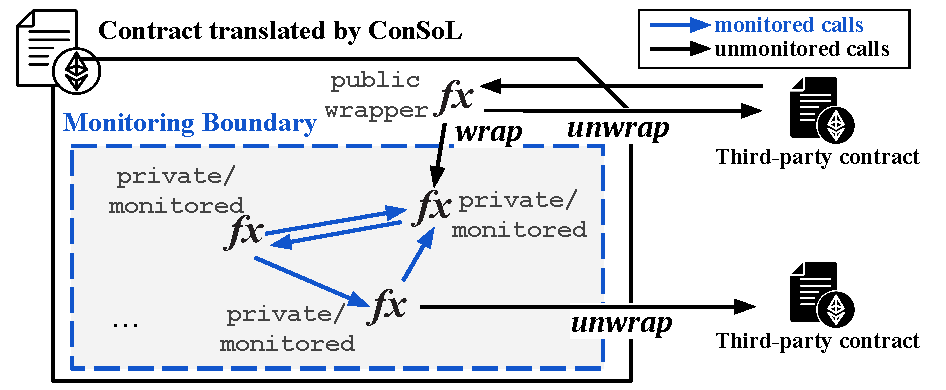
\includegraphics[width=0.85\linewidth]{monitoring_boundary.pdf}
	\vspace{-1mm}
	\caption{Monitoring boundary of guarded address calls.}
	\label{fig:monitor_bound}
	% \vspace{-1em}
\end{figure}

Additionally, a function $f$ with the same name and interface as the original function
is generated. This is used only for external calls (if the $f$ is public), which
does not observe our translated value representation for addresses.

The attachment of specifications to addresses is performed by $\mathit{attachSpec}$ 
at run-time, whose implementation depends on the representation of guarded addresses.

% \subsubsection*{\textbf{Translating Statements and Expressions}}
\bfpara{Translating Statements and Expressions.}
\lang translates statements and expressions in a recursive fashion (\Cref{fig:translation}). 
Most cases of statement translation are straightforward; they
recursively apply the translation to subcomponents.
Declared types $t$ are lifted to $t^\uparrow$
% , so that they can 
to
carry specifications.

For binary operations, we first recursively translate the operands, 
and apply $\mathit{unwrap}$ to the operands at run-time.
Since the attachment of specifications to address values may change the underlying
representing values, this is necessary to ensure our translation preserves the 
results of these operations. For example, consider the same address value $x$
attached with two different specifications $x_1$ and $x_2$. The programmer
should expect $x_1 == x_2$, which only holds after unwrapping.
In general, $\mathit{unwrap}$ should be applied when performing computation 
other than method calls over values.

Direct function calls are replaced with their guarded counterparts $f_\textit{guard}$ with arguments being translated recursively.
Address calls $\kappa(e_\mathit{addr}).f$ are replaced with calls to $\mathit{dispatch}^\kappa_f$, %\xx{grammar}
which takes the address value $e_\mathit{addr}$ in addition to the ordinary arguments as arguments.
The $\mathit{dispatch}$ inspects the specification provenance carried along with
the underlying address value, performs the corresponding checks before and after
the address calls.

% \subsubsection*{\textbf{Runtime Facilities}}
\bfpara{Runtime Facilities.}
Our translation works against a set of runtime functions, including
$\mathit{wrap}$ and $\mathit{unwrap}$ that convert value representations,
$\mathit{attachSpec}$ that bakes specification provenance into the underlying guarded address values, and
$\mathit{dispatch}$ that decodes specification provenance and performs corresponding
checked address calls. %\xx{checked calls?} 
Since $\mathit{dispath}$ makes address calls to external contract instances,
it applies $\mathit{unwrap}$ to arguments before interacting with worlds outside \lang's monitoring boundary.
Note that $\mathit{dispatch}$ is a family of functions that are specialized over the callee 
function $f$ and its interface $\kappa$.
In \Cref{sec:impl}, we describe the implementation of $\mathit{attachSpec}$ and $\mathit{dispatch}$.

% \subsubsection*{\textbf{A Concrete Example}}
\iffalse
Take the deposit function from \Cref{sec:examples-higher-order} as an example. The translated Solidity program is as follows.
\begin{lstlisting}[language=Consol]
deposit(token, amount) requires msg.sender == owner
where {
  IERC20(token).transferFrom(sender, addr, amount) returns (success)
  requires amount > 0   ensures success
}
\end{lstlisting}
\vspace{-0.25em}
\begin{lstlisting}
function deposit(address$^\uparrow$ token, uint amount) public {
  IERC20(token).transferFrom(...); // the call is now guarded
}
\end{lstlisting}
\fi

%\bfpara{A Concrete Example}
%\note{Yeah}\xx{???}

\subsection{Correctness} \label{sec:correctness}


Our translation preserves the semantics of the original program, in 
the sense that if the \lang-translated program does not raise \lang-related 
errors, then we observe the same result and state on the original program.

Moreover, \corelang guarantees that any violation will be detected 
(thus the execution will be reverted) \emph{within the 
boundary of the current contract}. 
\Cref{fig:monitor_bound} demonstrates the monitoring boundary of \corelang with the blue dashed scope.
It is straightforward to see invocations of top-level functions are redirected to
their guarded version, thus correctly monitored.
Therefore, our analysis focuses on on guarded addresses. % i.e., \textit{chainlink} in \Cref{fig:sturbyIntro}\xx{i.e., xxx in figure}\yy{added}\wac{No explanation of this spec on \textit{chainline} before this point}.
Once an address is attached with guards, there are three possible ways to unwrap it in
our translation: 
(1) the address value is used in primitive operations (e.g. comparing equality),
(2) the address value is returned to other contract instances via a public function 
(\Cref{fig:fun-translation}),
(3) the address value is passed as an argument (thus unwrapped by $\mathit{dispatch}$)
to other contract instances.
We say addresses in (2) and (3) escape our monitoring boundary, as demonstrated in \Cref{fig:monitor_bound}.
All other calls of guarded addresses stay in our boundary for effective monitoring. \looseness=-1

\begin{figure}[t]
	\centering
	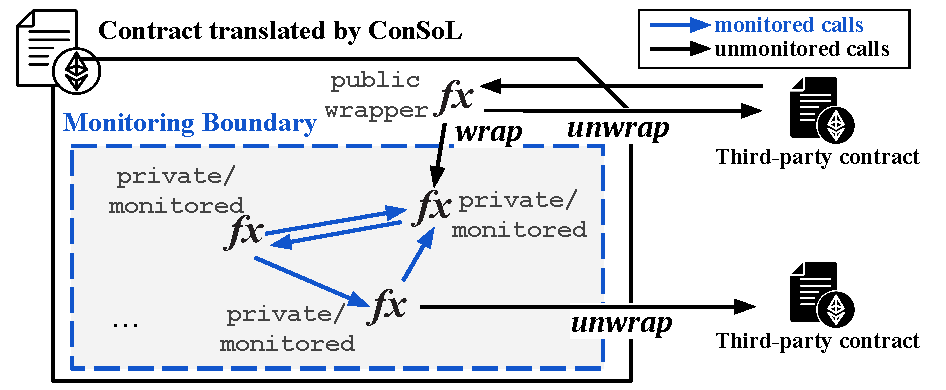
\includegraphics[width=0.85\linewidth]{monitoring_boundary.pdf}
	\vspace{-1mm}
	\caption{Monitoring boundary of guarded address calls.}
	\label{fig:monitor_bound}
	% \vspace{-1em}
\end{figure}

\renewcommand{\arraystretch}{0.8}

\begin{table}[t]
\centering
\caption{Summary of studied cases. \textit{LR} denotes LoC Reduced.}
\vspace{-1mm}
% \textit{Loss} denotes the monetary loss measured in US Dollars, and \textit{LR} denotes the percentage of lines from the assertion-based patched functions that have been translated into \lang annotations, in comparison to their original total lines.}
\small
\setlength{\tabcolsep}{2.5pt}
\label{tab:case}
\begin{tabular}{lcrlc}
\toprule
\multicolumn{1}{c}{\textbf{Project}} & \textbf{Date}     & \multicolumn{1}{c}{\textbf{Loss} (\$)} & \multicolumn{1}{c}{\textbf{Attack Type}} & \multicolumn{1}{c}{\textbf{LR}  (\%)} \\
\midrule
Umbrella~\cite{unbrellaHack}                    & 03-20-22 & 700K                     & Integer Over/Underflow                & 33.33                           \\
EFLeverVault~\cite{eflevervaultHack}                & 10-14-22 & 1M                       & Business Logic Flaw    & 25.00                           \\
N00d~\cite{n00dHack}                        & 10-26-22 & 29K                      & Reentrancy                      & 11.11                           \\
Dexible~\cite{dexibleHack}                     & 02-17-23 & 1.5M                     & Arbitrary External Call         & 11.76                           \\
SushiSwap~\cite{sushiSwapHack}                   & 04-09-23 & 3.3M                     & Unchecked User Input            & 54.55                           \\
SwaposV2~\cite{swaposv2Hack}                    & 04-16-23 & 468K                     & Erroneous Accounting            & 25.00                           \\
Unknown~\cite{unknownHack}               & 05-31-23 & 111K                     & Missing Slippage Check          & 30.00                           \\
Sturdy~\cite{sturbyHack}                      & 06-12-23 & 800K                     & Readonly Reentrancy            & 57.14                           \\
LEVUSDC~\cite{levusdcHack}                     & 06-15-23 & 105K                     & Access Control                  & 33.33                           \\
Bao~\cite{baoHack}                & 07-04-23 & 46K                      & Inflation Manipulate            & 83.33    \\
\bottomrule
\end{tabular}
\end{table}

It is worth noting that the user-provided condition expressions are also translated (\Cref{fig:fun-translation}).
This is deliberated to provide stricter semantics (known as the
``picky'' contract semantics \cite{DBLP:journals/jfp/BlumeM06}) to allow 
using guarded addresses to define conditions, which can capture more potential violations.

%translated by \lang passes all the runtime checks, 
%then the original \corelang program won't breach the attached specifications 
%when run in an identical state. \note{revisit}
% \yy{added}\note{correctness: if [p] does not have \lang-errors, then p runs without errors too.}

\section{Implementation and Optimizations}\label{sec:impl}

We implement \lang as a preprocessor of Solidity programs annotated with
\lang's specifications. Given an input program, \lang generates a Solidity
program following the translation outlined in \Cref{sec:model}.
The output programs can be compiled and deployed using off-the-shelf Solidity
toolchains without any further modification.
\lang is implemented with \code{solc-typed-ast}~\cite{solctypedast},
% the help of \note{X} parser, 
which can also reify a modified AST back to a Solidity program.
%\xx{the \lang spec is parsed with~\cite{antlr4}}

Our implementation handles Solidity features that are not covered by
the formalization, e.g., mappings, structs, and low-level calls.
Additionally, programmers can attach specifications to storage fields,
which can be desugared to core forms. This is useful to produce guarded
addresses at contract initialization time.

%\todo{syntax sugar: top-level initialization spec --> translate constant to immutable --> add function}

%\todo{what we didn't model in \Cref{sec:model}: mapping, structs, arrays, low-level calls, HO functions}
%Our current implementation does not handle inlined assembly. \todo{why}

%Contracts for higher-order functions are another future work when Solidity has 
%proper support for lambda expressions. Without such proper support from the base language,
%\todo{...}

% \subsubsection*{\textbf{Optimizations}} 
% \smallskip \noindent \textbf{Optimizations.}
\bfpara{Optimizations.}
The translation presented in \Cref{fig:translation} works with a set of runtime functions.
These functions cooperate with the runtime representation of guarded addresses.
We now discuss an optimized implementation that \emph{does not incur additional storage overhead}
in the generated code.

The optimization exploits the fact that the smallest unit for storage is 256 bits 
in the Ethereum Virtual Machine. Storing or loading for data smaller than 256 bits
incurs the same gas overhead as data of 256 bits.
However, the size of an address is 160 bits, which spares additional 96 bits that
can be used to encode specifications up to 96 predicates.
Therefore, we use \code{uint256} to represent guarded addresses, where the 96 MSB
encodes attached specifications and 160 LSB is preserved for addresses.

With this representation, our translation assigns numbers to conditions of addresses.
The correspondence between the assigned number and their runtime functions is emitted 
in the generated code.
Those runtime functions then can be easily implemented: The $\mathit{wrap}$ function coerces a 
\code{uint160} to \code{uint256}, and $\mathit{unwrap}$ function discards the 96 MSB of an \code{uint256} value.
The $\mathit{attachSpec}$ function only modifies the 96 MSB of a guarded address representation.
The $\mathit{dispatch}$ function can check which bits in the 96 MSB of the guarded addresses
are set, therefore knows which predicates to check.

The total number of conditions attached to addresses cannot exceed 96.
However, so far, we have not encountered real cases that need to use more than 96 address conditions. 
If with more conditions, our translation could fall back to the naive encoding discussed in \Cref{sec:translation}.

\iffalse
+ representing guarded address
+ eliminate redundant calls - the compiler should do so ... (e.g., from guarded to worker)
+ combining pre-/post-conditions in different functions (many functions share the same precondition), 
  to reduce the number of specs 
+ Syntax sugar?
\fi
%Question: where to place modifier?
\vspace{-5pt}
\section{Case Studies} \label{sec:case}

% + 10 cases, sourced from XXX, per type, and its corresponding defenses.
% + we shows that those defenses can be expressed with  a few lines of non-intrusive of \lang, decoupled from the main busness, making developers focus on the logic.
% + we start with xxx, and discussion more on two representive cases.

% In this section, we demonstrate
This section showcases \lang's the expressiveness and effectiveness
using 10 real-world smart contract attacks (\$8 million loss in total) and defenses. 
We first provide a comprehensive overview of our case study, then 
delve into two representative cases, illustrating
how \lang specifications concisely and non-intrusively express security defenses, 
% can be concisely expressed using a few non-intrusive \lang annotations and thereby 
decoupling from their primary business logic. % showcasing that \lang can facilitate development by alleviating interference between low-level checks and business logic.


\begin{figure}[t]
% \begin{subfigure}[t]{0.49\textwidth}
\centering
\begin{lstlisting}[language=Consol,numbers=left,stepnumber=1,xleftmargin=0.8em,numberstyle=\ttfamily\color{gray},numbersep=3pt,firstnumber=1]
$\HLBoxGreen{\mathit{IERC20(token).transferFrom(\_, \_, \_)\ returns\ (ret)\ requires\ ret}}$
\end{lstlisting}
\vspace{-0.45em}
\begin{lstlisting}[numbers=left,stepnumber=1,xleftmargin=1em,numberstyle=\ttfamily\color{gray},numbersep=3pt,firstnumber=2]
IERC20 public immutable token;
\end{lstlisting}
\vspace{-0.4em}
\begin{lstlisting}[language=Consol,numbers=left,stepnumber=1,xleftmargin=0.8em,numberstyle=\ttfamily\color{gray},numbersep=3pt,firstnumber=3]
$\HLBoxGreen{\mathit{withdraw(n,\ user)}}$
$\HLBoxGreen{\mathit{requires\ \_canOperate(msg.sender,\ user)}} \HLBoxRedUnderlined{\mathit{\&\&\ \_balances[user]\ >=\ n}}$
\end{lstlisting}
\vspace{-0.45em}
\begin{lstlisting}[numbers=left,stepnumber=1,xleftmargin=1em,numberstyle=\ttfamily\color{gray},numbersep=3pt,firstnumber=5]
function withdraw(uint256 n, address user) {
  $\HLBoxRed{\textcolor{gray}{\texttt{require(\_canOperate(msg.sender, user));}}}$
  _balances[user] = _balances[user] - n;
  $\HLBoxRed{\textcolor{gray}{\texttt{bool\ success =}}}$ token.transferFrom(address(this), user, n);
  $\HLBoxRed{\textcolor{gray}{\texttt{require(success)}}}$  
}
function deposit(uint256 n, address user) {
  $\HLBoxRed{\textcolor{gray}{\texttt{bool\ success =}}}$ token.transferFrom(user, address(this), n);
  $\HLBoxRed{\textcolor{gray}{\texttt{require(success);}}}$  
}
\end{lstlisting}
% \caption{The vulnerability in Umbrella project}
% \label{fig:integer_hack}
% \end{subfigure}
% \hfill
% \begin{subfigure}[t]{0.49\textwidth}
% \centering
% \begin{lstlisting}[language=Consol,numbers=left,stepnumber=1,xleftmargin=0.8em,numberstyle=\ttfamily\color{gray},numbersep=3pt,firstnumber=1]
% IERC20(token).transferFrom(_, _, _) returns (ret) requires ret
% \end{lstlisting}
% \vspace{-0.45em}
% \begin{lstlisting}[numbers=left,stepnumber=1,xleftmargin=1em,numberstyle=\ttfamily\color{gray},numbersep=3pt,firstnumber=2]
% IERC20 public immutable token;
% \end{lstlisting}
% \vspace{-0.45em}
% \begin{lstlisting}[language=Consol,numbers=left,stepnumber=1,xleftmargin=0.8em,numberstyle=\ttfamily\color{gray},numbersep=3pt,firstnumber=3]

% withdraw(n, user) 
% requires _canOperate(msg.sender, user) $\HLBox{\&\&\ \_balances[user] >= n}$
% \end{lstlisting}
% \vspace{-0.45em}
% \begin{lstlisting}[numbers=left,stepnumber=1,xleftmargin=1em,numberstyle=\ttfamily\color{gray},numbersep=3pt, firstnumber=6]
% function withdraw(uint256 n, address user) {
%   _balances[user] = _balances[user] - n;
%   token.transferFrom(address(this), user, n);
% }

% function deposit(uint256 n, address user) {
%   ...
%   token.transferFrom(user, address(this), n);
% }
% \end{lstlisting}
% \caption{\lang-fixed}
% \label{fig:integer_hack_fix}
% \end{subfigure}
\caption{Simplified code for Umbrella: The added \lang spec is highlighted in blue, 
eliminating the assertions (in red). The additional condition for the fix is underlined.}
\label{fig:integer}
\end{figure}






% To demonstrate the expressiveness and effectiveness of \lang, in this section, we investigate 10 real-world smart contracts attacks, and their corresponding defenses.
% We shows that those defenses can be expressed with  a few lines of non-intrusive \lang annotation and decoupled from the main business logic, easing the development by eliminating the interfers amongs security checks and core business.
% We first present the overall result of our case studies, and then discuss two representative cases.


% In this section, we examine several real-world attacks, to demonstrate how \lang can be used to consolidate smart contracts. 
% We now turn our attention to real-world cases and examine how \lang
% can be used to consolidate smart contract programs.
% These case studies are empirical evidence showing \lang is effective
% in preventing attacks.

% \vspace{-3mm}

\bfpara{Data and Methodology.}
%We study
% Our case studies comprise the examination of 
%10 real-world smart contract attacks 
% that resulted
%resulting in over
% a total loss exceeding 
%\$8 million loss.
The 10 attacks are sourced from a reputable blockchain incident database~\cite{defihacklabs},
which is widely used in the literature~\cite{DBLP:conf/icse/ZhangZXL23,DBLP:conf/icis/KeN22,DBLP:journals/iacr/ZhouXECWWQWSG22}.
\Cref{tab:case} summarizes these attacks,
where the first three columns present the projects' names, attack dates, and corresponding financial losses.
% the names of the projects, the dates, and the financial loss associated with each attack, respectively. 
Our collection covers 10 most frequent types of attacks (the 4th column) 
listed in the database.

We analyze each attack,
% For each attack, we investigate the attack process, 
identify the root cause, and pinpoint the vulnerable function. 
%Following this, 
We implement the most appropriate patch, 
% comprised of 
using low-level assertions (as suggested by postmortem incident reports from third-party auditors 
\cite{consensys,trailofbits}), and then migrate the patch using \lang. 
%highly-regarded security auditing 
% To verify the validity of
To validate the patches, we employ an Ethereum Archive Node~\cite{reth} to replay all 
historical transactions on both
patched contracts (assertion-based and \lang-based), 
ensuing legitimate transactions succeed 
while blocking the malicious ones.
% the malicious ones are blocked.

% Our case study consists of investigation of 10 real-world smart contract attacks sourced from a well-known blockchain incident database, which is widely used in literature.
% For each attack, we investigate the attack process and identify the root cause as well as the vulnerable function.
% After that, we apply the most proper patch written by low-level assertions (suggested by incident postmortems from well-reputated security auditing companies), and then rewrite the patched functions by \lang.
% To demonstrate the correctness of patches, we leverage an Ethereum archive node to replay all the historical transactions upon the two versions of patched contracts (by assertions and \lang).
% We ensure all the benign transactions can be successfully processed while the attacking one will be prevented. 
% 

% Table~\ref{tab:case} presents the summary of our case study. 
% The first three columns presents the names of projects, the dates, and the fund loss of each attack, respectively.
% The forth column denotes the types of attack.
% It is worthnoting that, to demonstrate that \lang can assist in developing defend against various types of attacks, the attacks under investigation belong to the most common 10 attack types suggested by the database.

\bfpara{Result Overview.}
% the type of attack. 
% It is noteworthy that, to 
% the development of 
All \lang-annotated programs successfully defend against these attacks. 
% The last column
Column ``LR'' in \Cref{tab:case} denotes the percentage of LoC reduced
from the assertion-patched functions after adopting \lang.
%translated into \lang specifications.
% , in comparison to their original total lines. 
%\xx{the definition ``in comparison... '' is confusing, removed. add back if it is wrong.}
% For instance, 20\% means 20\% LoC in a function can be expressed as specifications using \lang.
On average 36.5\% LoC in the assertion-patched functions can 
be expressed as specifications with \lang.
Since a substantial portion of these functions is dedicated to validation,
\lang appears to be an ideal tool to decouple validations from business logic,
hence improving readability and maintainability. \looseness=-1
% an average of approximately \xx{why approximate?} 36.5\% LoC can be converted into \lang specification, 
% This suggests that 
% , separate from the core logic. 
% Recall that, a
%A high LR indicates \lang's modular design effectively enhances readability and 
%maintainability and decouples the validation checks from core business logic. 
% As illustrated by \Cref{fig:sturbyIntro}, the extensive interference of validation checks and core business flow makes the development of secure code a challenging task. The more the validation logic can be separated from the core logic, the easier it becomes to develop secure code. 
%\zz{too verbose, revisit it later}\xx{revised}
% \zz{todo: a better way to justify why we choose this criterion.}
% Decoupling this validation logic contributes to a cleaner, more readable, and potentially more maintainable code structure.
% On the other hand, it is noteworthy that
\iffalse
% \xx{consider removing following content, or significantly simplify this}
Notably, 
N00d and Dexible projects have a relatively smaller proportion of validation code. 
% Upon further investigation, we find that 
This is because they 
% these two projects 
already adopt a style that maintains pre- and post-conditions, as demonstrated in the subsequent code.
\begin{lstlisting}
function fill(SwapRequest request) returns (SwapMeta) {
  preCheck(request, meta); // hand-crafted pre-conditons
  SwapMeta meta = ... // code related to the business flow
  require(meta.outAmount >= request.tokenOut.amount); }
\end{lstlisting}
This implies a deliberate intention on the part of the developers to have an effective and user-friendly mechanism to dictate and enforce contract behaviors.
However, due to the limited expressiveness of the vanilla Solidity, some security defenses still reside in the core function bodies, leading developers to overlook certain subtle cases.
It thereby underscores the motivation behind the development of \lang. 
\fi

% As shown in \Cref{tab:case}, on average, around 36.5\% lines of code can be converted into \lang annotations, indicating a large portion of code in functions are validation logic and not related to the core flow.
% Decoupling these validation helps lead to cleaner, more readable, and potentially more maintainable code. 
% Observe that N00d and Dexible have relatively small portion of validation code. 
% Further investigation indicates that these two projects are already written in a style of maintaining pre-/post-coditions, as indicated by the following code. 
% 
% It indicates the developer's intention of having an effective and convenient means to specify and enforce contract behaviors.
% However, due to the limited expressiveness of vanilla Solidity, a few security defenses still remain in the core function bodies, rendering the developers overlook some subtle cases.




\bfpara{Case 1: Integer Underflow.}
We use integer underflow, a notorious vulnerability type, as an example to demonstrate
\lang's effectiveness in expressing the defense. %preventing attacks.
% how \lang can facilitate development by minimizing the complexity of the code logic.
\Cref{fig:integer} depicts a simplified code snippet from the Umbrella project.
Specifically, the Umbrella project offers a staking service where users can stake and unstake their \texttt{token}s through the \texttt{deposit} (lines 11-14) and \texttt{withdraw} (lines 5-10) functions, respectively. 
%Profits are allocated to users who stake an ample amount of tokens for a sufficient duration, whose implementation is excluded from the code snippet for simplicity.
The \texttt{withdraw} function 
% initially verifies if \texttt{msg.sender} has the right to operate the fund of \texttt{user} (line 4), 
updates the \texttt{\_balances} of the user (line 7), transfers the staked tokens (line 8), and finally checks if the transfer is successful (line 9). 
We skip the detail of the \texttt{deposit} function, except for its operation involving the transfer of tokens (lines 12-13), as well as several other functions operating on token transfers for the sake of simplicity.

\renewcommand{\arraystretch}{0.8}
\begin{table}[t]
\centering
\caption{Gas consumption on vulnerable contracts in 
% dataset 
$\mathcal{D}_2$, patched with assertions and \lang.
GFI: gas fee increase (\$).
GIR: gas increase ratio after patching 
% on \lang-implemented contracts 
% compared 
to the original.
}
\vspace{-1mm}
\label{tab:case_gas}
\setlength{\tabcolsep}{4pt}
\small
\begin{tabular}{lccccc}
\toprule
\multicolumn{1}{c}{\multirow{2.2}{*}{\textbf{Project}}} & \multirow{2.2}{*}{\textbf{\#Tx}} & \multicolumn{2}{c}{\textbf{by Assertions}} & \multicolumn{2}{c}{\textbf{by \lang}} \\ 
\cmidrule(lr){3-4} \cmidrule(lr){5-6}
\multicolumn{1}{c}{}                         &                       & \textbf{GFI (\$)}               & \textbf{GIR (\%)}               & \textbf{GFI (\$)}                    & \textbf{GIR (\%)}                    \\
\midrule
Umbrella~\cite{unbrellaHack}                                    & 3                     & 0.012             & 0.151             & 0.021                  & 0.249                  \\
EFLeverVault~\cite{eflevervaultHack}                                 & 13                    & 0.043             & 0.094             & 0.050                  & 0.109                  \\
N00d~\cite{n00dHack}                                         & 46                    & 0.022             & 1.656             & 0.027                  & 2.099                  \\
Dexible~\cite{dexibleHack}                                      & 54                    & 0.048             & 0.088             & 0.126                  & 0.230                  \\
SushiSwap~\cite{sushiSwapHack}                                    & 3                     & 0.479             & 4.820             & 0.511                  & 5.147                  \\
SwaposV2~\cite{swaposv2Hack}                                     & 1                     & 0.019             & 0.188             & 0.025                  & 0.244                  \\
Unknown~\cite{unknownHack}                                      & 10                    & 0.018             & 0.010             & 0.434                  & 0.269                  \\
Sturdy~\cite{sturbyHack}                                       & 19                    & 1.138             & 1.221             & 1.139                  & 1.223                  \\
LEVUSDC~\cite{levusdcHack}                                      & 7                     & 0.051             & 0.143             & 0.054                  & 0.152                  \\
Bao~\cite{baoHack}                                          & 15                    & 0.004             & 0.036             & 0.007                  & 0.069                   \\
\midrule
\textbf{Avg.} & 17.1 &	0.183 &	0.841 &	0.239 &	0.979\\
\bottomrule
\end{tabular}
\end{table}
% \vspace{-2mm}

\smallskip
\noindent
\underline{\textit{Attack.}}
The vulnerability resides at line 5, where the attacker attempts to withdraw a large quantity of their staked tokens. 
This action induces an integer underflow 
% \footnote{This project is written in Solidity 0.7.5, which does not check overflow and underflow.} 
in \texttt{\_balance[user]-n}, leading to an anomalously large \texttt{\_balance[user]} for the attacker. 
Consequently, the attacker is able to transfer as many tokens as they wish. \looseness=-1

\smallskip
\noindent
\underline{\textit{\lang-Patch.}}
One effective patch to fix this vulnerability is to guard \texttt{withdraw} with
a pre-condition \texttt{\_balance[user] > n}.
However, considering the extensive security validations that must be placed 
around every invocation of \texttt{token.transferFrom},
there is a heightened risk that developers overlook these subtle 
checks for integer underflow.
As depicted in \Cref{fig:integer}, \lang's solution to this challenge is 
to attach specifications to both function \texttt{withdraw} and calls of 
address \texttt{token} (line 1).
As the result, there is no need to repeatedly write validation code
checking the same condition in multiple locations, since the storage address is persistently guarded, thanks to our whole-program translation.  

This strategy reduces the number of duplicated assertions 
currently interspersed across various invocation sites.
Moreover, by moving all validation logic from \texttt{withdraw} function 
to modularly defined specifications, it enhances the readability of both the business and validation logic.
% become more readable.

%developers can readily assess the 
%validity of the logic without the risk of oversight.

%enables developers to attach 
%a specification directly to \texttt{token} (line 1) thereby expel the 



% \Cref{fig:integer_hack} presents the code snippet of the Umbrella project, which is significantly simplified for illustrative purpose.
% Specifically, Umbrella project provides a staking service where users can stake and unstake their \texttt{token}s via \texttt{\textbf{function} deposit} (lines 10-14) and \texttt{\textbf{function} withdraw} (lines 3-8), respectively.
% Profit will be provided if users stake a sufficient amount of tokens for enough time, whose corresponding implementation is not related to the vulnerability and hence omitted.
% With the \texttt{withdraw} function, the code first checks the \texttt{msg.sender} can operate the fund of \texttt{user} (line 4), update the \texttt{\_balances} of the user (line 5), transfers out the staked tokens (line 6), and check whether the transfer succeeds (line 7).
% For function \texttt{deposit}, we ignore its detailed implementation except its operation upon transferring tokens (line 12).
% Note that there are many other functions operating on token transfers but being omitted for simplicity. 
% 
% The vulnerabilty lies at line 5, where the attacker try to withdraw a large amount of staked tokens of him, which causes an integer overflow (or underflow) of \texttt{\_balance[user] - n} and result in a significantly large \texttt{\_balance[user]} for the attacker. 
% The attacker can then transfer as many tokens as he wants.



\bfpara{Case 2: Readonly Reentrancy.} 
Readonly reentrancy represents another notorious class of vulnerabilities.
%that has led to significant financial losses in the blockchain ecosystem. 
% Conventional reentrancy can typically be mitigated by employing a Reentrancy Guard~\cite{XXX}\zz{cite} (typically implemented as a modifier). 
% However, a newly discovered variant of this vulnerability, referred to as \textit{readonly reentrancy}, continues to pose considerable threats. 
We use the Sturdy~\cite{sturdy} project 
to illustrate how \lang can enhance readability and potentially help prevent such vulnerabilities. %\zz{readability?}

\smallskip \noindent \underline{\textit{Attack.}}
\Cref{fig:sturby_buggy} shows the simplified \texttt{getPrice} function from the Sturdy contract, 
which determines the price of the Sturdy token. 
The returned price of \texttt{getPrice} function is proportional to Ether price,
which ratio is informed by \texttt{ORACLE.getRate} (line 7).
However, the return value of \texttt{ORACLE.getRate} (shown in \Cref{fig:oracal}) can be manipulated by attackers,
exploiting the fact that \texttt{getRate} (line 1, \Cref{fig:oracal}) returns a ratio of \texttt{this.balance / totalSupply}. 
%The \texttt{withdraw} function (lines 2-7) enables users to withdraw their deposited Ether from the contract. 
The ratio is manipulated by providing a malicious callback to a \texttt{withdraw} function (line 2-6),
which first employs a low-level call to transfer the requested Ether amount back to \texttt{msg.sender}.
Nevertheless, this low-level call allows \texttt{msg.sender} to callback \texttt{getPrice} 
before \texttt{withdraw} finishes its update to \texttt{totalSupply}.
At this moment, the nominator of the ratio \texttt{this.balance} has been lowered by the Ether transfer,
causing \texttt{getRate} yields an abnormally low value.
This, in turn, leads to \texttt{getPrice} returning an inflated value.
Given that smart contracts rely on precise token prices, such miscalculations 
due to this vulnerability can result in significant financial losses. 

\smallskip
\noindent \underline{\textit{\lang-Patch.}}
The fix to this issue is to cross-validate 
\texttt{getPrice} with the latest Sturdy price, which can be accessed 
from \texttt{ORACLE.get}-\texttt{LatestPrice}. 
In \lang, this check can be concisely expressed by a post-condition (lines 2-3 in \Cref{fig:sturby_fix}).

%The reentrancy vulnerability in this scenario arises due to the callback 
%to \texttt{msg.sender} invoked at line 4 in \Cref{fig:oracal}. 
%In the callback, \texttt{msg.sender} can maliciously call \texttt{getPrice} 
%function in \Cref{fig:sturby_buggy}, which subsequently calls \texttt{getRate} (\Cref{fig:oracal}). 
% This function allows  before the callback returns. 
% The attacker manipulates this by calling the \texttt{getPrice} function in \Cref{fig:sturby_buggy}, which subsequently calls \texttt{getRate} in \Cref{fig:oracal}.
%Note that at this point, the state of \texttt{ORACLE} is only partially updated since 
%\texttt{this.balance} already decreases at line 4 while \texttt{totalSupply} is not yet 
%updated (to be updated at line 6).

% As \texttt{this.balance} reduces automatically at the start of the \texttt{msg.sender.call}, and \texttt{totalSupply} decreases only after the callback, \texttt{getRate} returns an abnormally high value when it's called. 
%For example, an attacker could sell a token worth \$1 for \$1 million.

% This function first retrieves the price of Ether (i.e., the native cryptocurrency of the Ethereum network) (lines 2-3) from ChainLink~\cite{XXX}\zz{cite}, checks if the returned value is up-to-date (lines 4-5), and then calculates the exchange rate from Ether to its own token, thereby determining the token's price (line 7). 
% Note that lines 9-10, which were introduced to patch the vulnerability, are not part of the original code.



\begin{figure}[t]
\centering
\begin{lstlisting}[numbers=left,stepnumber=1,xleftmargin=1em,numberstyle=\ttfamily\color{gray},numbersep=3pt]
function getRate() { return this.balance / totalSupply; }
function withdraw() nonReentrancy {
  uint balance = this.balance
  msg.sender.call{value: balanceOf[msg.sender]}();
  balanceOf[msg.sender] = 0;
  totalSupply -= amount * totalSupply / balance;  }
\end{lstlisting}
\caption{The code snippet of \texttt{ORACLE} used by Sturdy.}
\label{fig:oracal}
\end{figure}




\iffalse
\subsection{Readonly Reentrancy}
\todo{XX: background section TODO: explain callback function in background and what is tokens, how nonreentranct modifier works}
\wac{I think it's better to introduce reentrancy here.}
% Market.xyz readonly reentrancy attack.
% Transfer return value not checked.
% Li.fi attack: Arbitrary call to untrusted code (low-level call).

% \paragraph{Severity} talk about severity for each case


The first type of attack that \lang can prevent is \textit{readonly reentracy}.
A reentrancy attack refers to an attacker hijacking the control flow of a vulnerable function and re-entering the same function or same contract before the vulnerable function's execution finishes.
Such control flow hijacking breaks the atomicity of a function execution and can lead to catastrophic consequences.
Modern contracts prevent reentrancy attacks by attaching \code{nonReentrant} guard \todo{cite} to functions so that a global lock is acquired and released before and after the function execution.
However, a \code{readonly} (or \code{view}) function can only read from but not modify the contract's storage. 
Due to its nature, it can't carry a \code{nonReentrant} modifier, which is implemented via a lock shared by all functions within the same contract, stored in the contract's storage \todo{(refer to the background section)}. 
Readonly reentrancy attacks occur when a \code{readonly} (or \code{view}) function is invoked during the execution of another function that is modifying the contract's state, which can potentially lead to a situation where stale data is read.
 % In DeFi transactions, while they are atomic off-chain, multi-legged transactions may exist in an ``in-between state", which is vulnerable to reentrancy.
% Consequently, functions or contracts depending on the returned value may be exploited, resulting in undesirable or malicious behavior such as overpayment of protocol fees, rate manipulation, or incorrect pricing.

\subsubsection{Attack} We use the Sturdy attack~\cite{sturbyHack} to illustrate this type of attack and how \lang can prevent it. The hack takes three entities, balancer, lending contract (victim), and the attacker.
\paragraph{Balancer} is an automated portfolio manager and liquidity provider. It manages token pools, offering APIs for creating pools, trading tokens, and depositing or withdrawing tokens from the pool while imposing trading fees. Additionally, Balancer offers APIs that enable users to access exchange rates among tokens. 
\paragraph{Lending Contract (victim)} is a type of smart contract that provides lending services, allowing users to lend their digital assets in return for interest. To borrow assets from the lending contract, users must provide collateral with a value exceeding the borrowing amount. The borrowed assets and the collateral can be different tokens (for instance, using USDC as collateral to borrow ETH).
\paragraph{Attacker} The Attacker (A) exploits the Victim contract (V) by borrowing tokens from it. Let's assume that A has collateral in the form of token1, which is worth the value of $v_1$ at V, and intends to borrow a certain amount of token2, worth $v_2$ from V. Here, $v_2$ is typically strictly less than $v_1$ at the current exchange rate accessed from Balancer (B). By manipulating the exchange rate in B between token1 and token2, A is able to borrow token2 worth an excessive value $v_2'$ from V, where $v_2'$ significantly exceeds $v_1$, and worth \$\todo{xx} in the hack to Sturdy Finance. 


We'll break down the exploit within a single transaction, conducted by A, in a step-by-step manner.  Prior to the attack transaction, A initially deposits a small amount of token1 into V as collateral to enable him/herself to borrow token2 from V later in the attack. 

At the beginning of the hack transaction, A leverages a flash loan, enabling the borrowing of a vast amount of assets as long as these borrowed assets are paid back within the same transaction.
A then deposits this large quantity of assets in the form of token2 \xx{correct? or doesn't matter} into B and immediately withdraws them via the \code{exitPool} function (line 6 \Cref{fig:sturbyHack}), which carries a \code{nonReentrant} modifier to prevent reentrant access.
At line 8, the \code{exitPool} function calls the callback function of the recipient (i.e., A) before updating the pool token balance (line 9). Within this callback function, A proceeds to borrow a substantial amount of token2 from V. Given that some amount of token1 has been deposited by A at V, V needs to verify the exchange rate between token1 and token2 to ensure the borrowed value is less than the collateral's value. This is done via the \code{\_get} function in  \Cref{fig:sturby_buggy} which retrieves the exchange rate by calling B's \code{getRate} API (\Cref{fig:sturbyHack}), where the contract B is reentered.  However, 
\code{getRate} 
% is a \code{view} function, and thus 
fails to fetch the latest exchange rate, because the rate is affected by the balance, which isn't updated until line 9 executes after returning from the callback function. As a result, \code{getRate} provides an incorrect exchange rate, significantly lower\todo{lower or higher?} than its true value. Consequently, A manages to borrow from V an amount of token2 that is far more valuable than the collateral, with a portion of it paid back to the flash loan.


\subsubsection{Solution} 
While it might seem straightforward to address this for Balancer by stopping using the \code{getRate} function as \code{readonly}, it's more crucial and urgent for the victim, the lending contract, to find a solution. One approach is to specify a post-condition for the \code{get} function, as shown in \Cref{fig:sturby_fix}. This post-condition prevents the attack by checking the Automated Market Maker (AMM) invariant\todo{cite}, which is violated during the reentrancy calls.



\begin{figure}[t]
\begin{lstlisting}[numbers=left,stepnumber=1,xleftmargin=1em,numberstyle=\ttfamily\color{gray},numbersep=3pt]
function getRate() public view returns (uint256) {
  uint256 _poolTokenBalance = _getPoolTokenBalance(); // not uptated
  return _calculateRate(_poolTokenBalance);
}

function exitPool(address sender, address recipient, 
  uint256 amount) nonReentrant external {
  (bool success, ) = recipient.call{value: amount}(""); // reentrancy
  _updatePoolTokenBalance(amount);
}
\end{lstlisting}

\caption{A Simplified Demonstration of an Readonly Reentrancy: Balancer Contracts}
\label{fig:sturbyHack}
\end{figure}
\fi

\iffalse
\subsection{Arbitrary External Call}


\begin{figure}[t]
\begin{lstlisting}[numbers=left,stepnumber=1,xleftmargin=1em,numberstyle=\ttfamily\color{gray},numbersep=3pt]
function fill(SwapTypes.SwapRequest calldata request, 
SwapMeta memory meta) external onlySelf returns (SwapMeta memory)  {
  //some checks
  for(uint i=0;i<request.routes.length;++i) {
    SwapTypes.RouterRequest calldata rr = request.routes[i];
    IERC20(rr.routeAmount.token).safeApprove
        (rr.spender, rr.routeAmount.amount);
    (bool s, ) = rr.router.call(rr.routerData);  // vulnerable
    ...
    }
  ...
  require(meta.outAmount >= request.tokenOut.amount,
  "Insufficient output generated");
}
\end{lstlisting}

\caption{A Simplified Demonstration of an Arbitrary External Call Bug: Dexible Contracts}
\label{fig:dexibleHack}
\end{figure}



\begin{comment}
\begin{figure}[t]
\begin{lstlisting}[numbers=left,stepnumber=1,xleftmargin=1em,numberstyle=\ttfamily\color{gray},numbersep=3pt]
struct SwapData {
  address callTo;
  bytes callData;
  ...
}
function swap(bytes32 transactionId, SwapData calldata _swap) 
  internal {
  ... // some balance check
  meta.outAmount = request.tokenOut.token.balanceOf(address(this));
  (bool success, bytes memory res) = _swap.callTo.call{
    value: nativeValue
  }(_swap.callData);
  if (!success) {
    string memory reason = LibUtil.getRevertMsg(res);
    revert(reason);
  }
  ...
}

\end{lstlisting}

\caption{A Simplified Demonstration of an Arbitrary External Call Bug: LiFi Contracts}
\label{fig:lifi_example}
\end{figure}

\begin{figure}[t]
\label{fig:lifi_solution}
\begin{lstlisting}[language=Consol]
swap (transactionId, _swap) 
requires {(_swap.callTo == XXX && _swap.callData[:4] == YYY) || ...}
\end{lstlisting}

\begin{lstlisting}[language=Consol]
swap (transactionId, _swap) 
where { _swap.callTo.call(data) returns (success, res)
    requires {_swap.callTo == XXX && data[:4] == YYY) || ...}
    ensure {success}
}
\end{lstlisting}
\caption{\lang Specifications for LiFi attack.}
\label{fig:lifi_solution}
\end{figure}

\end{comment}



The second type of attack that \lang can prevent is unsafe arbitrary external calls, 
which allows an attacker to make a contract call to any arbitrary function. 
We illustrate this type of attack with the Dexible attack\todo{cite}.

\subsubsection{Attack} 
% ~\cite{lifiHack}. 
\Cref{fig:dexibleHack} shows a simplified version of the vulnerable function within the Dexible contract, 
the \texttt{fill} function,
% function,  an internal function that facilitates
which facilitates asset swapping within a smart contract. 
% \xx{why is the library called libswap not contract lifi}

To call the \code{fill} function, users need to provide \code{request} and \code{meta}. The  \code{request} is an object of \code{SwapTypes.SwapRequest}, 
which contains an entry \code{routes}, a tuple of \code{SwapTypes.RouterRequest}, each of which describes a step in the swap operation including \todo{xxx} \todo{meta ...}
% , which contains entries \texttt{callTo} and \texttt{callData}. 
% A user can make a 
Transactions are made by invoking \texttt{rr.router.call} with the provided \code{rr.routerData}. Since there is no check on the \code{rr}, this enables users to make the Dexible contract (the victim contract) call other arbitrary functions, with the victim contract being the message sender instead of the users (e.g., attackers) themselves. 

Dexible incorporates an \textit{approve} mechanism \xx{correct?}, where users can give control of their funds to it so that Dexible has permission to transfer their funds. Specifically, consider Bob (the victim user) grants Dexible approval to manage his funds in ERC20. Alice (the attacker), exploits this approval by calling the \code{fill} function with a \code{request}, where \code{request.routes} consists a \code{SwapTypes.RouterRequest} object, say \code{rr}, with \code{rr.router} set to USDC, and \code{rr.routerData} is \code{transferFrom(Bob, Alice, 100)}. Consequently, Alice executes a transaction that transfers funds (i.e., 100 USDC tokens) from Bob's account to hers. \xx{correct?}


\subsubsection{Solution} A straightforward approach to fix the vulnerability in the contract is to incorporate guards for the \code{rr.router} and \code{rr.routerData} (line xx and xx). This could be done with a series \code{require} statements, e.g., enforce the value of \code{bytes4(rr.routerData[:4])}, therefore prevent arbitrary calls by maintaining a "whitelist".  With \lang, this can be efficiently accomplished using the following spec:

\begin{lstlisting}[language=Consol]
fill(request, meta) returns (meta)
requires _checkRequest(request)
ensures meta.out >= request.tokenOut.amount
\end{lstlisting}

In this case, \lang enables the decoupling of decalring (\spec{\_checkRequest}) and usage (within the \code{fill} function) of the specifications. Furthermore, our specification can replace the \code{require} statement in line 10 (\Cref{fig:dexibleHack}) with an \spec{ensures}-clause to enforce this post-condition.
\fi



\begin{comment}
    \paragraph{Solution} After the attack, LiFi implemented a whitelist mechanism, which allows calls only to pre-approved contracts and functions. Such a blocking mechanism requires xxxx \todo{shortcomings}. \lang can effectively prevent such attack with a single-place specification. We provide two solutions with \lang in Fig.~\ref{fig:lifi_solution}.

The first solution is by adding a pre-condition to the first-order argument (Section~\todo{3.1}), i.e., \spec{\_swap}. With this spec, \lang conducts a check on its entries, \spec{callTo} and \spec{callData}, via a \spec{require}-clause that ensures the contracts and functions being called are indeed on the whitelist. 
The second solution treats \spec{\_swap.callTo} as a higher-order argument (Section~\todo{3.2}) and enforces its properties via a \spec{where}-clause. 

Functionally, both solutions perform checks on the enforced conditions on the contract being called. The only distinction is the time the checks are performed. With the first spec, the check is conducted immediately upon entering the \texttt{swap} function, as the spec is on the argument of the function. With the second spec, the check is performed when \texttt{\_swap.callto.call} is actually invoked. 
Both the specs are effective in preventing the attack. We offer these as two alternative solutions to underscore the flexibility and adaptability of \lang.

\end{comment}




\iffalse
\subsection{Return Value Not Check}
\fi

\iffalse
\begin{table}[t]
\centering
\caption{Summary of case studies. \textit{Loss} denotes the monetary loss measured in US Dollars, and \textit{LR} denotes the percentage of lines from vulnerable functions that are converted into behavioral contracts, relative to the original total lines in these functions.}
\small
\setlength{\tabcolsep}{3.5pt}
\label{tab:case}
\begin{tabular}{lcrlc}
\toprule
\multicolumn{1}{c}{\textbf{Project}} & \textbf{Date}     & \multicolumn{1}{c}{\textbf{Loss}} & \multicolumn{1}{c}{\textbf{Attack Type}} & \multicolumn{1}{c}{\textbf{LR (\%)}} \\
\midrule
Umbrella~\cite{unbrellaHack}                    & 03-20-22 & 700K                     & Integer Overflow                & 33.33                           \\
EFLeverVault~\cite{eflevervaultHack}                & 10-14-22 & 1M                       & Business Logic Flaw    & 25.00                           \\
N00d~\cite{n00dHack}                        & 10-26-22 & 29K                      & Reentrancy                      & 11.11                           \\
Dexible~\cite{dexibleHack}                     & 02-17-23 & 1.5M                     & Arbitrary External Call         & 11.76                           \\
SushiSwap~\cite{sushiSwapHack}                   & 04-09-23 & 3.3M                     & Unchecked User Input            & 54.55                           \\
SwaposV2~\cite{swaposv2Hack}                    & 04-16-23 & 468K                     & Erroneous Accounting            & 25.00                           \\
Unknown~\cite{unknownHack}               & 05-31-23 & 111K                     & Missing Slippage Check          & 30.00                           \\
Sturdy~\cite{sturbyHack}                      & 06-12-23 & 800K                     & Read Only Reentrancy            & 57.14                           \\
LEVUSDC~\cite{levusdcHack}                     & 06-15-23 & 105K                     & Access Control                  & 33.33                           \\
Bao~\cite{baoHack}                & 07-04-23 & 46K                      & Inflation Manipulate            & 83.33    \\
\bottomrule
\end{tabular}
\end{table}
\fi

\iffalse
\begin{table}
	\centering
	\caption{Summary of case studies.
 % \wac{The dForce link is broken. I changed it.}\xx{we should use reference (not hyperlink)?}\wac{Not sure. Maybe you are right.} 
 }
	\label{tab:case}
	\begin{tabular}{cccc}
		\toprule
		\textbf{Type} & \textbf{Case} & \textbf{Date} & \textbf{Loss} \\
		\midrule
		\multirow{4}{*}{\rotatebox[origin=c]{90}{\begin{tabular}{@{}c@{}}Readonly \\Reentrancy\end{tabular}}}
		& Sentiment~\cite{sentimentHack} & 04/05/23 & \$1M \\
		& dForce~\cite{dforceHack} & 02/10/23 & \$3.65M \\
		& MidasCapital~\cite{midascapitalHack} & 01/16/23 & \$650K \\
		& Market.xyz~\cite{marketxyzHack} & 10/24/22 & \$220K \\

		\midrule

		\multirow{10}{*}{\rotatebox[origin=c]{90}{Arbitrary External Call}}
		& MIMSpell~\cite{mimspellHack} & 06/20/23 & \$17K \\
		& Phoenix~\cite{phoenixHack} & 03/07/23 & \$100K \\
		& RevertFinance~\cite{revertFinanceHack} & 02/18/23 & \$30K \\
		& Dexible~\cite{dexibleHack} & 02/12/23 & \$1.5M \\
		& CowSwap~\cite{cowswapHack} & 02/07/23 & \$120K \\
		& Rubic~\cite{rubicHack} & 12/25/22 & \$1.5M \\
		& BrahTOPG~\cite{brahtopgHack} & 11/09/22 & \$89K \\
		& MEV\_0ad8~\cite{mev0ad8Hack} & 11/08/22 & \$282K \\
		& Rabby~\cite{rabbyHack} & 10/11/22 & \$200K \\
		& Li.Fi~\cite{lifiHack} & 03/20/22 & \$570K \\

		% \midrule

		% \multirow{5}{*}{\rotatebox[origin=c]{90}{\begin{tabular}{@{}c@{}}Return Value\\Not Check\end{tabular}}}
		% & & & \\
		% & & & \\
		% & \href{https://medium.com/@QubitFin/protocol-exploit-report-305c34540fa3}{Qubit} & 01/28/22 & \$80M \\
		% & & & \\
		% & & & \\
		\bottomrule
	\end{tabular}
\end{table}
\fi

% reentrancy: Checks, Effects, Interactions naturally?

% \newpage
\section{Gas Efficiency} \label{sec:perf}
\label{sec:eval}


% \wac{Do we organize evaluation using RQs?}

% \subsection{Performance Overhead}
% \begin{itemize}
% 	\item Gas cost
% 	\item DeFi projects with source code and test cases.
% 	\item Migrate ``Securing smart contract with runtime validation'' data (with ERCxxx invariant).
% \end{itemize}

\begin{table*}[th]
    \centering
    \small
    \caption{Average transaction gas consumption on contracts of dataset $\mathcal{D}_1$~\cite{DBLP:conf/pldi/LiCL20}. 
    GIR: gas increase ratio on \lang-implemented contracts compared to the original.
    LR: percentage of lines in functions that are expressed in \lang specifications.}
    % \vspace{-1mm}
    \label{tab:solythesis_evaluation}
 %    \resizebox{\linewidth}{!}{% 
 %    \begin{tabular}{ccccccccccccccccccccccccc}
	% \toprule
 %        \textbf{Contract}  & \textbf{BEC} & \textbf{USDT} & \textbf{ZRX} & \textbf{THETA} & \textbf{INB} & \textbf{HEDG} & \textbf{DAI} & \textbf{EKT} & \textbf{XIN} & \textbf{HOT} & \textbf{SWP} & \textbf{VOTE} & \textbf{DOZ} & \textbf{MCHH} & \textbf{CC} & \textbf{CLV} & \textbf{LAND} & \textbf{CARDS} & \textbf{KB} & \textbf{TRINK} & \textbf{PACKS} & \textbf{BKC} & \textbf{EGG} \\
 %        \midrule
 %        \textbf{Original}  & 114,726 & 62,426 & 51,468 & 51,540 & 53,738 & 53,941 & 53,696 & 51,911 & 51,375 & 51,525 & 55,728 & 118,293 & 255,038 & 138,034 & 133,651 & 150,692 & 134,750 & 133,787 & 133,765 & 133,497 & 156,071 & 143,674 & 134,252 \\
 %        \textbf{\lang} & 115,555 & 63,382 & 51,468 & 51,895 & 54,090 & 54,160 & 53,960 & 52,258 & 51,727 & 51,566 & 55,952 & 118,411 & 255,558 & 138,576 & 134,188 & 151,440 & 135,281 & 134,175 & 134,156 & 134,017 & 156,459 & 144,013 & 134,460 \\
 %        \textbf{GIR (\%)}   & 0.72 & 1.53 & 0.00 & 0.69 & 0.66 & 0.41 & 0.49 & 0.67 & 0.69 & 0.08 & 0.40 & 0.10 & 0.20 & 0.39 & 0.40 & 0.50 & 0.39 & 0.29 & 0.29 & 0.39 & 0.25 & 0.24 & 0.16 \\
 %        \textbf{LR (\%)} & 39.10 &      30.83 &     0.00 &     38.89 &   38.89 &    50.00 &   50.00 &   40.83 &   34.44 &   44.44 &     50.00 &      20.83 & 43.19 &     33.33 &   35.71 &    41.67 &     33.33 &      33.81 &   37.05 &        35.71 &      33.33 &    37.05 &    37.50 \\
 %        \bottomrule
 %    \end{tabular}
 %    }

% \resizebox{\linewidth}{!}{% 
    \begin{tabular}{ccccccccccccccccccccccccc}
	\toprule
        \textbf{Contract}  & \textbf{BEC} & \textbf{USDT} & \textbf{ZRX} & \textbf{THETA} & \textbf{INB} & \textbf{HEDG} & \textbf{DAI} & \textbf{EKT} & \textbf{XIN} & \textbf{HOT} & \textbf{SWP} & \textbf{VOTE} \\
        \midrule
        \textbf{Original}  & 114,726 & 62,426 & 51,468 & 51,540 & 53,738 & 53,941 & 53,696 & 51,911 & 51,375 & 51,525 & 55,728 & 118,293 \\
        \textbf{\lang} & 115,555 & 63,382 & 51,468 & 51,895 & 54,090 & 54,160 & 53,960 & 52,258 & 51,727 & 51,566 & 55,952 & 118,411 \\
        \textbf{GIR (\%)}   & 0.72 & 1.53 & 0.00 & 0.69 & 0.66 & 0.41 & 0.49 & 0.67 & 0.69 & 0.08 & 0.40 & 0.10 \\
        \textbf{LR (\%)} & 39.10 &      30.83 &     0.00 &     38.89 &   38.89 &    50.00 &   50.00 &   40.83 &   34.44 &   44.44 &     50.00 &      20.83  \\
        \bottomrule
    \end{tabular}
    % }
    \vspace{3pt}
    % \resizebox{\linewidth}{!}{% 
    \begin{tabular}{ccccccccccccc}
	\toprule
        \textbf{Contract} & \textbf{DOZ} & \textbf{MCHH} & \textbf{CC} & \textbf{CLV} & \textbf{LAND} & \textbf{CARDS} & \textbf{KB} & \textbf{TRINK} & \textbf{PACKS} & \textbf{BKC} & \textbf{EGG} \\
        \midrule
        \textbf{Original} & 255,038 & 138,034 & 133,651 & 150,692 & 134,750 & 133,787 & 133,765 & 133,497 & 156,071 & 143,674 & 134,252  \\
        \textbf{\lang} & 255,558 & 138,576 & 134,188 & 151,440 & 135,281 & 134,175 & 134,156 & 134,017 & 156,459 & 144,013 & 134,460  \\
        \textbf{GIR (\%)}   & 0.20 & 0.39 & 0.40 & 0.50 & 0.39 & 0.29 & 0.29 & 0.39 & 0.25 & 0.24 & 0.16 \\
        \textbf{LR (\%)} & 43.19 &     33.33 &   35.71 &    41.67 &     33.33 &      33.81 &   37.05 &        35.71 &      33.33 &    37.05 &    37.50 \\
        \bottomrule
    \end{tabular}
    % }
\end{table*}
% \vspace{-2mm}

\lang offers developers a powerful tool to decouple the specifications from the business logic.
However, the adoption of \lang may induce runtime overhead in terms of gas consumption.
% In this section, 
% With the optimizations (Section~\ref{sec:impl}), 
In this section,
we show that the overhead induced in using \lang to declare function specifications is minimal.

% \noindent\textbf{Dataset}: 
\bfpara{Dataset.}
We use two datasets to evaluate the gas efficiency of \lang.
First, we leverage the dataset collected by Li et al.~\cite{DBLP:conf/pldi/LiCL20}, which consists of 23 contracts in ERC20, ERC721, and ERC1202 standards ($\mathcal{D}_1$).
Second, we leverage the contracts of the 10 real-world attacks collected in Section~\ref{sec:case} ($\mathcal{D}_2$).
We collect the historical transactions on Ethereum invoking the corresponding vulnerable 
contracts to evaluate the gas consumption of \lang.

% \noindent\textbf{Baseline and comparison}:
\bfpara{Baseline and Methodology.}
The baseline we compare with \lang is the contracts where low-level assertions are directly implemented as pre-/post-conditions in the function body or around address calls.
Specifically, for dataset $\mathcal{D}_1$, the baseline is the original contracts collected by Li et al.~\cite{DBLP:conf/pldi/LiCL20}.
Specifications are already implemented in the original contracts using \texttt{require} or \texttt{assert} statements.
To evaluate the gas efficiency of \lang, for each contract, we manually re-implement it by extracting the assertion-based pre-/post-conditions and expressing them in \lang specifications, while preserving the original contract logic.
% The dataset is equipped with transactions calling each contract, which allows us to evaluate the gas efficiency of \lang by executing these transactions on the original contracts and the reimplemented version of them using \lang.
We leverage the test cases (transactions) provided by Li et al.~\cite{DBLP:conf/pldi/LiCL20} to execute and evaluate the gas consumption of the baseline and \lang.
For dataset $\mathcal{D}_2$, we manually patch the vulnerable contracts using assertions and \lang, respectively.
We replay all historical transactions on Ethereum that cover the patched functions and measure the gas consumption of the baseline and \lang-patched version.

% \noindent\textbf{Results}:
\bfpara{Results.}
Table~\ref{tab:solythesis_evaluation} shows the comparison of gas consumption on dataset $\mathcal{D}_1$.
Row \textit{Original} and \textit{\lang} show the average transaction gas consumption on the original contract and \lang-implemented contract, respectively.
The gas increase ratio of \lang-implemented version compared to the original contract is given in the third row \textit{GIR}.
The results show that such overhead of \lang specifications is minimal, only 0.43\% more gas on average for each contract. 

Table~\ref{tab:case_gas} shows the comparison of gas consumption on dataset $\mathcal{D}_2$.
Column \textit{GFI} and \textit{GIR} give the average increased gas fee (in US dollar) and gas consumption increase ratio of transactions on the patched contract compared to the original vulnerable contract.
Column \textit{by Assertions} and \textit{by \lang} shows the GFI and GIR on the baseline (assertion-patched contracts) and \lang-patched contracts.
Column \textit{\#Tx} gives the total number of historical transactions executed on the patched functions.
Similar to experiments on dataset $\mathcal{D}_1$, patching vulnerable contracts using \lang specifications only has minimal gas overhead (avg. \$0.239), corresponding to at most \$1.2 more transaction fees.
Compared to baseline, \lang specifications also induce a small increase in gas, thanks to the optimizations to avoid additional storage overhead in the generated code (\Cref{sec:impl}).
% , but the overhead is small.
% given that \lang provides a powerful linguistic means to attach specifications decoupled from contract logic implementations. 
% Note that, we adopt optimizations to avoid additional storage overhead in the generated code (\Cref{sec:impl}).
The overhead is induced by the additional private function call generated in the translation of functions with \lang specifications.
Such overhead is minimal since the private function calls are compiled into cheap JUMP instructions.
\looseness=-1

On dataset $\mathcal{D}_1$ we also report the percentage of lines in original functions that are expressed as \lang specifications (Column \textit{LR} in Table~\ref{tab:solythesis_evaluation}).
Similar to the results in Table~\ref{tab:case}, a large portion of code in functions can be extracted as \lang specifications.
This indicates the \lang is effective in separating specifications from business logic in functions.

% \wac{Below are deprecated}
% Row \textit{Gas Increase} gives the increase ratio of average gas consumption for transactions on each contract.

% To measure how many behavioral contracts can be extracted from each function, we also measure the average lines of code (LOC) reduced for each function by decoupling pre-conditions and post-conditions from the function business logic.
% For instance, 20\% means 20\% lines of code in a function can be specified as function behavioral contracts using \lang.
% The row \textit{LOC Reduced} shows the average percentage of each function that can be extracted as behavioral contracts using \lang.
% On average for each function, 36.51\% lines of code are specifications of pre- and post-conditions, which can be specified using \lang.
% The result indicates that a large portion of code in functions is not related to business logic. 
% If the function behaviors can be specified and enforced using \lang, developers can focus more on the main business logic with clean and maintainable code, reducing programming errors in the implementation.
% \zz{need to revist, given the newly-introduced case study section. e.g., we already explain what Reduced LoC is in that section.}

% \subsection{Readability}
% \begin{itemize}
% 	\item Number hunk of code to measure the efforts to fix a bug.
% 	\item Number of tokens required to fix.
% \end{itemize}


\section{Related Work} \label{sec:related}

% \subsubsection*{\textbf{Behavioral Contracts and Runtime Verification}}
\bfpara{Behavioral Contracts.}
The Eiffel programming language pioneered the ``design-by-contract'' methodology \cite{DBLP:books/ph/Meyer91, DBLP:conf/tools/Meyer98a}, 
advocating the idea of setting clear expectations between software components 
right at the outset of software development.
\citet{DBLP:conf/icfp/FindlerF02} proposed to extend the notion of behavioral contracts 
to higher-order functions.
\lang borrows ideas from contracts for higher-order functions to monitor
address specifications, given their same higher-order essence.
An interesting future work of \lang is to extend it with higher-order temporal contracts \cite{DBLP:conf/icfp/DisneyFM11},
which would be particularly useful for smart contract programs.
%While our work, in its current iteration, focuses on first-order and higher-order behaviors of smart contracts, we anticipate the foundational endeavor paves the way for consideration of more expressive behaviors.

\iffalse
This is most related to a security mechanism called stack inspection, which is implemented in systems like \texttt{Java} to prevents access from untrusted components to resources protected by trusted components \cite{DBLP:conf/popl/FournetG02, DBLP:conf/sp/WallachF98}. 
However, \lang propagates address specifications down the stack and performs check at call sites while stack inspection inspects the entire call stack before accessing certain resources.
\fi

\iffalse
袁老板related work写得太好了不忍心删 hhh
The landscape of behavioral contracts has seen notable advances over the past decades.
Arguably one of the pioneering efforts in assertion-based contracts is 
the ``design-by-contract'' methodology \cite{DBLP:books/ph/Meyer91, DBLP:conf/tools/Meyer98a} 
as realized in the \texttt{Eiffel} programming language. 
It advocates the idea of setting clear expectations between software components 
right at the outset of software development.
Pushing the boundaries, \texttt{DrScheme} incorporates an assertion monitoring system 
to support contracts for higher-order functions \cite{DBLP:conf/icfp/FindlerF02}.
%
To support temporal contracts on top of higher-order contracts, \citet{DBLP:conf/icfp/DisneyFM11} formalizes the behavior of imperative higher-order functions as a sequence of events, namely calls to other functions and the matching returns, and imposes the delineated contracts over the event sequences.
%
More recently, a behavioral contract, drawing inspiration from a static "size-change" termination verification approach \cite{DBLP:conf/popl/LeeJB01}, is developed to enforce termination \cite{DBLP:conf/pldi/NguyenGTH19}, which otherwise cannot be checked directly during runtime as a canonical liveness property.
%
% a form of liveness properties, i.e. something good will happen eventually.
% This work only considers safety property, i.e. monitoring and preventing something bad will not happen.


\lang not only takes inspiration from these prior works but also proposes a distinct feature -- persistent monitoring of address specifications.
Recall that smart contract is a domain where programs have direct economic outcome but often suffers from attacks due to its open-world distributed nature. \lang provides programmers a convenient way to specify the intended behavior of external functions, which otherwise is beyond their control.
% \lang also stands out among other behavioral contract system in its unique handling The distinct nature of smart contracts compared to normal programs poses real-world challenges that \lang tackles through its specification monitoring system, as discussed throughout the paper.
%
% Notably, by attaching specification to address values, \lang is able to enforce checks upon entry and exit of external functions, which is beyond programmers' control.
%
This is most related to a security mechanism called stack inspection, which is implemented in systems like \texttt{Java} to prevents access from untrusted components to resources protected by trusted components \cite{DBLP:conf/popl/FournetG02, DBLP:conf/sp/WallachF98}. 
%
However, \lang propagates address specifications down the stack and performs check at call sites while stack inspection inspects the entire call stack before accessing certain resources.

While our work, in its current iteration, focuses on first-order and higher-order behaviors of smart contracts, we anticipate the foundational endeavor paves the way for consideration of more expressive behaviors.
% A closely related work to our temporal contracts and monitoring is interface automata \cite{DBLP:conf/sigsoft/AlfaroH01}.
\fi

% \subsubsection*{\textbf{Smart Contracts}}



% survey \cite{DBLP:journals/csur/TolmachLLLL22}
% core calculus of Solidity-like languages \cite{DBLP:conf/sp/JiaoK0S0020, Sergey2021, DBLP:conf/esorics/BartolettiGM19, DBLP:conf/fc/CrafaPZ19}
\bfpara{Smart Contracts.}
%Researchers have made efforts to securing smart contracts from many aspects.
Runtime validation of smart contracts is the most relevant direction to \lang.
\citet{DBLP:conf/pldi/LiCL20} propose a technique to translate user specified 
contract-level invariants into solidity code via delta update and delta check.
\citet{chen2022declarative} propose a declarative smart contract language, 
which also inserts runtime checks after compilation.
\citet{DBLP:conf/edcc/EllulP18} propose violation resolution procedures in runtime verification when specifications are violated.
In contrast, \lang provides finer-grained property checking with function-level checks and persistent address monitoring.

Orthogonal to \lang, static analysis and verification of smart contract programs are intensively studied.
\citet{DBLP:journals/csur/TolmachLLLL22} survey the use of formal specification and verification techniques
in securing smart contracts.
Statically checked refinement types \cite{coblenzObsidianSaferBlockchain2017,DBLP:journals/pacmpl/TanMLDF22}
allow developers to write specifications as part of types.
\citet{DBLP:journals/pacmpl/BramEMSS21} propose a specification methodology to 
capture the intended behaviors of contracts under development, as well as external 
unverified contracts.
\cite{DBLP:journals/pacmpl/GrossmanAGMRSZ18} works only on callback-related vulnerabilities that \lang can effectively prevent.
Researchers have also proposed works mining high-level semantics from contracts~\cite{liu2022finding,liu2022invcon}.
Recent studies have also focused on modeling Solidity semantics
\cite{DBLP:conf/sp/JiaoK0S0020, Sergey2021, DBLP:conf/esorics/BartolettiGM19, DBLP:conf/fc/CrafaPZ19}, and analyze flaws and vulnerabilities using pre-defined oracles~\cite{DBLP:journals/pacmpl/SmaragdakisGLTT21,DBLP:journals/pacmpl/GrechKJBSS18, DBLP:conf/pldi/Pirlea0S21, ghaleb2022etainter,liao2023smartstate, DBLP:journals/pacmpl/AlbertGRRRS20, DBLP:conf/pldi/BrentGLSS20}, focusing on aspects such as insecure payment~\cite{DBLP:journals/pacmpl/WangZS19}, 
% gas-related~\cite{ghaleb2022etainter}, 
and access control~\cite{ghaleb2023achecker}.
% , and callback~\cite{DBLP:journals/pacmpl/AlbertGRRRS20}, and composite vulnerabilities~\cite{DBLP:conf/pldi/BrentGLSS20}.
% Moreover, several empirical studies 
% \cite{renEmpiricalEvaluationSmart2021,durieuxEmpiricalReviewAutomated2020,DBLP:conf/icse/ZhangZXL23,DBLP:journals/tse/ZhangWCLLLL23} 
% have been conducted to evaluate contract analysis techniques.
% Compared to static approaches, 
In contrast, \lang is a programmer-oriented language extension and supports expressive specifications to conduct runtime verification.
% allows developers to express specifications that are checked at runtime.

% Solythesis~\cite{DBLP:conf/pldi/LiCL20}, leveraging delta instrumentation strategy, conducts runtime validation with little overhead, focusing only on contract-level global invariants. 



% \todo{recent se work}


% \xx{----split---}

% SPCon\cite{liu2022finding}, static (role mining) and dynamic detects potential permission bugs 

% InvCon \cite{liu2022invcon} dynamic invariant detection

% \cite{zheng2023turn} limitations of existing reentrancy detection tools (false positive), only detect call.value()

 % \cite{ghaleb2022towards} study show limitations (false positive), propose a static tool to reduce fp

 
% DeCon~\cite{chen2022declarative},  a declarative programming language specifying contract-level properties

% runtime verification \cite{DBLP:conf/edcc/EllulP18}
% runtime validation, reduce overhead of runtime checks \cite{DBLP:conf/pldi/LiCL20}

% Harvey: greybox fuzzer ~\cite{wustholz2020harvey}: gen transaction seq, and fuzz on seq

% ItyFuzz~\cite{shou2023ityfuzz} snap-shot based. identify state, dataflow analysis. 

% Smartian~\cite{choi2021smartian} fuzzing via static + dynamic data flow analysis


% SmartDagger~\cite{liao2022smartdagger} static, cross-contract vulnerability detection

% \cite{ren2021making} effort to make Smart Contract Development More Secure and Easier via better code-suggestion algo, integrating testing tool,

% MANDO-GURU~\cite{nguyen2022mando}, DL-based vul detection (call graph and control flow graph)
% security analyzer \cite{DBLP:conf/pldi/BrentGLSS20} detect composite information flow violations (static)

% nondeterminisitic payment bugs \cite{DBLP:journals/pacmpl/WangZS19} with information flow tracking (static)

% behavioral simulation to verify smart contracts \cite{DBLP:conf/pldi/BeillahiCEE20}

% formal and modular specification of smart contracts \cite{DBLP:journals/pacmpl/BramEMSS21}

% refinement types \cite{DBLP:journals/pacmpl/TanMLDF22}

% static analysis to infer ownership and commutativity summaries, for parallelism \cite{DBLP:conf/pldi/Pirlea0S21}

% callbacks \cite{DBLP:journals/pacmpl/AlbertGRRRS20, DBLP:journals/pacmpl/GrossmanAGMRSZ18} (1.static 2. static + dynamic)

% reduce gas consumption 
% gas-focused vulnerabilities (exploit undesired behavior when a contract runs out of gas) via control-flow analysis-based decompiler\cite{DBLP:journals/pacmpl/GrechKJBSS18}

% static analysis of Ethereum \cite{DBLP:journals/pacmpl/SmaragdakisGLTT21}



\section{Conclusion}

In this paper, we propose a specification and monitoring system, \lang,
for the Solidity smart contract programming language.
\lang supports attaching and enforcing specifications for both
top-level functions and address values.
\lang persistently monitors address calls via a whole-program
transformation, which ensures any violation of address call conditions
in the current contract scope is captured.
We examine the effectiveness and gas efficiency using 10 real-world attacks.
By replaying existing attack transactions, \lang-patched contracts successfully
defend the attack with only 0.98\% more gas consumption.

% vs FanLong 0.43%
% ERC20/ERC721/ERC1202 invaranits 0.43\%

%\section*{Acknowledgement}
\newpage
\bibliographystyle{ACM-Reference-Format}
\bibliography{10_references}

\end{document}

% Local Variables:
% TeX-engine: luatex
% TeX-master: t
% End:
